\section{Geometric Deep Learning Models}

Having thoroughly studied various instantiations of our Geometric Deep Learning blueprint (for different choices of domain, symmetry group, and notions of locality), we are ready to discuss how enforcing these prescriptions can yield some of the most popular deep learning architectures.

Our exposition, once again, will not be in strict order of generality. We initially cover three architectures for which the implementation follows nearly-directly from our preceding discussion: convolutional neural networks (CNNs), group-equivariant CNNs, and graph neural networks (GNNs).

We will then take a closer look into variants of GNNs for cases where a graph structure is not known upfront (i.e. unordered sets), and through our discussion we will describe the popular Deep Sets and Transformer architectures as instances of GNNs.

Following our discussion on geometric graphs and meshes, we first describe equivariant message passing networks, which introduce explicit geometric symmetries into GNN computations. Then, we show ways in which our theory of geodesics and gauge symmetries can be materialised within deep learning, recovering a family of intrinsic mesh CNNs (including Geodesic CNNs, MoNet and gauge-equivariant mesh CNNs).

Lastly, we look back on the grid domain from a \emph{temporal} angle. This discussion will lead us to recurrent neural networks (RNNs). We will demonstrate a manner in which RNNs are translation equivariant over temporal grids, but also study their stability to time warping transformations. This property is highly desirable for properly handling long-range dependencies, and enforcing class invariance to such transformations yields exactly the class of gated RNNs (including popular RNN models such as the LSTM or GRU). %Given that we aim to study time warping invariance in greater detail (and not just describe a model class), this subsection will be longer than the others. 

While we hope the above canvasses most of the key deep learning architectures in use at the time of writing, we are well aware that novel neural network instances are proposed daily. Accordingly, rather than aiming to cover every possible architecture, we hope that the following sections are illustrative enough, to the point that the reader is able to easily categorise any future Geometric Deep Learning developments using the lens of invariances and symmetries.

\subsection{Convolutional Neural Networks}
\label{sec:cnnsec}

Convolutional Neural Networks are perhaps the earliest and most well known  example of deep learning architectures following the blueprint of Geometric Deep Learning outlined in Section~\ref{sec:gdl_blueprint}. 
%
%
% ====
%
In Section \ref{sec:grids_euclidean} we have fully characterised the class of linear and local translation equivariant operators, given by 
convolutions ${\bf C(\thetab)}{\bf x} = {\bf x} \star \thetab$ with a localised filter $\thetab$\marginnote{Recall, ${\bf C}(\boldsymbol{\theta})$ is a \emph{circulant} matrix with parameters $\boldsymbol{\theta}$.}. 
Let us first focus on scalar-valued (`single-channel' or `grayscale') discretised images,  
%${\bf x}$ (having a single channel), 
where 
the domain is the grid $\Omega = [H] \times [W]$ with $\mathbf{u} = (u_1, u_2)$ and ${\bf x} \in \gX(\Omega, \R)$.

Any convolution with a compactly supported filter of size $H^f \times W^f$
can be written as a linear combination of 
generators $\thetab_{1,1}, \dots, \thetab_{{H^f,W^f}}$, given for example by the unit peaks $\boldsymbol{\theta}_{vw}(u_1, u_2) = \delta(u_1 - v, u_2 - w)$. Any local linear equivariant map is thus expressible as\marginnote{Note that we usually imagine $\vec{x}$ and $\boldsymbol{\theta}_{vw}$ as 2D matrices, but in this equation, both $\vec{x}$ and $\boldsymbol{\theta}_{vw}$ have their two coordinate dimensions \emph{flattened} into one---making $\vec{x}$ a vector, and $\vec{C}(\boldsymbol{\theta}_{vw})$ a matrix.} %directional derivatives $\thetab_{ij}(u_1,u_2) = \delta(u_1, u_2) - \delta(u_1-i,u_2-j), (i,j) \neq (0,0) $ plus the local average $\thetab_{0}(u_1,u_2) = \Delta^{-2}$. % \taco{I guess delta here is a function that equals 1 at (0,0) and 0 elsewhere? Could also mean 1 when u1 = u2, or it could be the Dirac delta which is infinite at zero... Maybe clarify. Also if my first guess is correct, is this really a basis? Can we express the filter which is 1 in the center and 0 elsewhere, i.e. delta(u1, u2)? Finally, just using a basis of delta peaks on each pixel might be more intuitive than directional derivatives?}
%\joan{Yes, here we used directional derivatives as analogy with graphs, in which derivative filters (Adjacency being lowpass filter and Laplacian being high-pass) are intrinsically defined. Correct I missed the average in the family of generators }
\begin{equation}
    \mathbf{F}(\mathbf{x}) = \sum_{v=1}^{H^f}\sum_{w=1}^{W^f} \alpha_{vw} \mathbf{C}(\thetab_{vw})\mathbf{x}~, 
\end{equation}
which, in coordinates, corresponds to the familiar 2D convolution (see Figure \ref{fig:2dconv} for an overview):
\begin{figure}
     \centering
     \includegraphics[width=0.7\linewidth]{figures/2d_conv.pdf}
     \caption{The process of convolving an image $\vec{x}$ with a filter $\vec{C}(\boldsymbol{\theta})$. The filter parameters $\boldsymbol{\theta}$ can be expressed as a linear combination of generators $\boldsymbol{\theta}_{vw}$.}
     \label{fig:2dconv}
\end{figure}
\begin{equation}\mathbf{F}(\mathbf{x})_{uv}= \sum_{a=1}^{H^f}\sum_{b=1}^{W^f} {\alpha}_{ab} x_{u+a, v+b}~.
\end{equation}
Other choices of the basis $\boldsymbol{\theta}_{vw}$ are also possible and will yield equivalent operations (for potentially different choices of $\alpha_{vw}$). A popular example are \emph{directional derivatives}: $\thetab_{vw}(u_1,u_2) = \delta(u_1, u_2) - \delta(u_1-v,u_2-w), (v,w) \neq (0,0) $ taken together with the local average $\thetab_{0}(u_1,u_2) = \frac{1}{H_fW_f}$. In fact, directional derivatives can be considered a grid-specific analogue of diffusion processes on graphs, which we recover if we assume each pixel to be a node connected to its immediate neighbouring pixels in the grid.

When the scalar input channel is replaced by multiple channels (e.g., RGB colours, or more generally an arbitrary number of \emph{feature maps}), the convolutional filter becomes a {\em convolutional tensor} expressing arbitrary linear combinations of input features into output feature maps. In coordinates, this can be expressed as 
%
\begin{equation}
\label{eq:basiccnnlayer}
\mathbf{F}(\mathbf{x})_{uvj}= \sum_{a=1}^{H^f}\sum_{b=1}^{W^f}\sum_{c=1}^M {\alpha}_{jabc} x_{u+a, v+b, c}~,~ j\in[N]~,
\end{equation}
%
where $M$ and $N$ are respectively the number of input and output channels. 
This basic operation encompasses a broad class of neural network architectures, which, as we will show in the next section, have had a profound impact across many areas of computer vision, signal processing, and beyond. Here, rather than dissecting the myriad of possible architectural variants of CNNs, we prefer to focus on some of the essential innovations that enabled their widespread use.  



\paragraph{Efficient multiscale computation} 
As discussed in the GDL template for general symmetries, extracting translation invariant features out of the convolutional operator $\mathbf{F}$ requires a non-linear step.\marginnote{\includegraphics[width=\linewidth]{figures/relu.pdf}\\ ReLU, often considered a `modern' architectural choice, was already used in the Neocognitron \citep{fukushima1982neocognitron}. Rectification is equivalent to the principle of demodulation, which is fundamental in electrical engineering as the basis for many transmission protocols, such as FM radio; and also has a prominent role in models for neuronal activity.} %so that the energy captured along each sub-band $\thetab_{ij}$ is mapped towards the low-frequencies
Convolutional features are processed through a non-linear %rectification stage, 
\emph{activation function} $\sigma$, acting element-wise on the input---i.e., $\sigma: \gX(\Omega) \to \gX(\Omega)$, as $\sigma(\mathbf{x})(u) = \sigma(\mathbf{x}(u))$. Perhaps the most popular example at the time of writing is the Rectified Linear Unit (ReLU): $\sigma(x) = \max(x, 0)$. %, or other choices of activation function. 
This non-linearity effectively \emph{rectifies} the signals, pushing their energy towards lower frequencies, and enabling the computation of high-order interactions across scales by iterating the construction.

Already in the early works of \cite{fukushima1982neocognitron} and \cite{lecun1998gradient}, CNNs and similar architectures 
%Since the early days from Fukushima and LeCun, CNN architectures 
had a multiscale structure, where after each convolutional layer (\ref{eq:basiccnnlayer}) one performs a grid coarsening 
$\mathbf{P} : \gX(\Omega) \to \gX(\Omega')$, where the grid $\Omega'$ has coarser resolution than $\Omega$. 
This enables 
multiscale filters with effectively increasing receptive field, yet retaining a constant number of parameters per scale. 
%
Several signal coarsening %or  
strategies $\mathbf{P}$ (referred to as \emph{pooling}) may be used, the most common are %possible: either %by %explicitly 
applying a low-pass anti-aliasing filter (e.g. local average) followed by grid downsampling, or non-linear max-pooling. 
%
%
%Inspired by neuroscience, 

In summary, a `vanilla' CNN layer can be expressed as the composition of the basic objects already introduced in our Geometric Deep Learning blueprint:
\begin{equation}
    \mathbf{h} = \mathbf{P}(\sigma(\mathbf{F}( \mathbf{x})))~,
\end{equation}
i.e. an equivariant linear layer $\mathbf{F}$, a coarsening operation $\mathbf{P}$, and a non-linearity $\sigma$. It is also possible to perform translation invariant \emph{global} pooling operations within CNNs. Intuitively, this involves each pixel---which, after several convolutions, summarises a \emph{patch} centered around it---\emph{proposing} the final representation of the image\marginnote{CNNs which only consist of the operations mentioned in this paragraph are often dubbed ``all-convolutional''. In contrast, many CNNs \emph{flatten} the image across the spatial axes and pass them to an MLP classifier, once sufficient equivariant and coarsening layers have been applied. This loses translation invariance.}, with the ultimate choice being guided by a form of aggregation of these proposals. A popular choice here is the average function, as its outputs will retain similar magnitudes irrespective of the image size \citep{springenberg2014striving}.

Prominent examples following this CNN blueprint (some of which we will discuss next) are displayed in Figure \ref{fig:cnn_drawn_plot}.

\begin{figure}
    \centering
    \includegraphics[width=0.85\textwidth]{figures/lenet.pdf}
    \includegraphics[width=0.85\textwidth]{figures/alexnet.pdf}
    \includegraphics[width=0.85\textwidth]{figures/resnet.pdf}
    \includegraphics[width=0.85\textwidth]{figures/Unet.pdf}
    \caption{Prominent examples of CNN architectures. \textbf{Top-to-bottom}: LeNet \citep{lecun1998gradient}, AlexNet \citep{krizhevsky2012imagenet}, ResNet \citep{he2016deep} and U-Net \citep{ronneberger2015u}. Drawn using the PlotNeuralNet package \citep{haris2018}.}
    \label{fig:cnn_drawn_plot}
\end{figure}
%role of depth
\paragraph{Deep and Residual Networks}
A CNN architecture, in its simplest form, is therefore specified by hyperparameters $(H^f_k, W^f_k, N_k, p_k )_{k \leq K}$, with $M_{k+1} = N_k$ and $p_k=0,1$ indicating whether grid coarsening is performed or not. While all these hyperparameters are important in practice, a particularly important  question is to understand the role of depth $K$ in CNN architectures, and what are the fundamental tradeoffs involved in choosing such a key hyperparameter, especially in relation to the filter sizes ($H_k^f, W_k^f$). 

While a rigorous answer to this question is still elusive, mounting empirical evidence collected throughout the recent years suggests a favourable tradeoff towards deeper (large $K$) yet thinner (small $(H^f_k, W^f_k)$) models \marginnote{
Historically, ResNet models are predated by \emph{highway networks} \citep{srivastava2015highway}, which allow for more general \emph{gating} mechanisms to control the residual information flow.}. In this context, a crucial insight by \cite{he2016deep} was to reparametrise each convolutional layer to model a \emph{perturbation} of the previous features, rather than a generic non-linear transformation:
\begin{equation}
    \mathbf{h} = \mathbf{P}\left(\mathbf{x} + \sigma(\mathbf{F}(\mathbf{x})) \right)~.
\end{equation}
The resulting \emph{residual} networks provide several key advantages over the previous formulation. In essence, the residual parametrisation is consistent with the view that the deep network is a discretisation of an underlying continuous dynamical system, modelled as an ordinary differential equation (ODE)\marginnote{In this case, the ResNet is performing a Forward Euler discretisation of an ODE: $\dot{\mathbf{x}} = \sigma( \mathbf{F}(\mathbf{x}))$}. Crucially, learning a dynamical system by modeling its velocity turns out to be much easier than learning its position directly. In our learning setup, this translates into an optimisation landscape with more favorable geometry, leading to the ability to train much deeper architectures than was possible before. As will be discussed in future work, learning using deep neural networks defines a non-convex optimisation problem, which can be efficiently solved using gradient-descent methods under certain simplifying regimes. The key advantage of the ResNet parametrisation has been rigorously analysed in simple scenarios \citep{hardt2016identity}, and remains an active area of theoretical investigation. 
Finally, Neural ODEs \citep{chen2018neural} are a recent popular architecture that pushes the analogy with ODEs even further, by learning the parameters of the ODE $\dot{\mathbf{x}} = \sigma( \mathbf{F}(\mathbf{x}))$ directly and relying on standard numerical integration. 

%\michael{This is also the case for GNNs, which are a discretization of a nonlinear diffusion PDE} \petar{skipping for now, as discussed with Michael}

%Normalization 
\paragraph{Normalisation} 
Another important algorithmic innovation that boosted the empirical performance of CNNs significantly is the notion of \emph{normalisation}. In early models of neural activity, it was hypothesised that neurons perform some form of local `gain control', where the layer coefficients $\mathbf{x}_{k}$ are replaced by $\mathbf{\tilde{x}}_{k} = \sigma_k^{-1} \odot (\mathbf{x}_{k} - \mu_k)$. Here, $\mu_k$ and $\sigma_k$ encode the first and second-order moment information of $\mathbf{x}_k$, respectively. Further, they can be either computed globally or locally.

In the context of Deep Learning, this principle was widely adopted through the \emph{batch normalisation} layer \citep{ioffe2015batch}\marginnote{We note that normalising activations of neural networks has seen attention even before the advent of batch normalisation. See, e.g., \cite{lyu2008nonlinear}.}, followed by several variants \citep{ba2016layer,salimans2016weight,ulyanov2016instance,cooijmans2016recurrent,wu2018group}. 
Despite some attempts to rigorously explain the benefits of normalisation in terms of better conditioned optimisation landscapes \citep{santurkar2018does}, a general theory that can provide guiding principles is still missing at the time of writing.  

\paragraph{Data augmentation}
While CNNs encode the geometric priors associated with translation invariance and scale separation, they do not explicitly account for other known transformations that preserve semantic information, e.g lightning or color changes, or small rotations and dilations. A pragmatic approach to incorporate these priors with minimal architectural changes is to perform \emph{data augmentation}, where one manually performs said transformations to the input images and adds them into the training set.

Data augmentation has been empirically successful and is widely used---not only to train state-of-the-art vision architectures, but also to prop up several developments in self-supervised and causal representation learning \citep{chen2020simple,grill2020bootstrap,mitrovic2020representation}. However, it is provably sub-optimal in terms of sample complexity \citep{mei2021learning}; a more efficient strategy considers instead architectures with richer invariance groups---as we discuss next.

%TODO: discuss Preserving Orientation: contrast this with the GNN setting. 

% ====

% To define a convolutional operator, we will consider the case of 2D inputs (i.e. single-channel images), $\vec{X}\in\mathbb{R}^{h\times w}$. Let $\vec{K}\in\mathbb{R}^{n\times m}$ be a small \emph{kernel matrix} (typically, $n = m = 3$ in modern neural network architectures). The kernel is overlaid in all possible ways
% over the input (see Figure \ref{fig:2dconv}), recording sums of elementwise products to create a
% new image, $\vec{X}'$:\marginnote{It should be noted that this approach is actually cross‐correlation rather than the convolution; but, for purposes of machine learning, the two are equivalent.}
% \begin{equation}
%     x'_{ab} = \sum_{i=1}^n\sum_{j=1}^m k_{ij}x_{a+i-1,b+j-1}
% \end{equation}
% The image is typically padded with sufficiently many zeroes on the edges, to ensure that the size of the output matches the size of the input.

% Moving from here to a convolutional \emph{layer} requires a few extensions. If the input has multiple channels, the kernel matrix is \emph{extended} in the channel dimension to match the input. This \emph{kernel tensor} specifies a single output channel. Each output channel requires a separate kernel tensor. Lastly, a channel‐specific bias and nonlinearity may be applied to obtain the final output image (sometimes known as a \emph{feature map}). 

% In summary, to process an input image $\vec{X} \in \mathbb{R}^{h\times w\times d}$ using a convolutional layer computing $d'$ channels, we require a kernel tensor $\vec{K}\in\mathbb{R}^{n\times m\times d\times d'}$ and a bias vector $\vec{b}\in\mathbb{R}^{d'}$, and proceed as follows:\marginnote{\includegraphics[width=\linewidth]{figures/fullconv.png}}
% \begin{equation}
%     x'_{abc} = \sigma\left(b_c + \sum_{i=1}^n\sum_{j=1}^m\sum_{k=1}^d k_{ijkc}x_{a+i-1,b+j-1,k}\right)
% \end{equation}

% This layer clearly exploits the structure present in an image, with neighbouring pixels
% influencing each other far more strongly than ones on opposite corners. The operator is
% also \emph{translation equivariant}, as required for grids: as the same kernels are applied identically across each image patch, we are encoding a structural bias that a feature of interest is important, no matter where it occurs in the image.

% Often, we are interested in computing outputs on the level of \emph{entire} images. Hence it is useful to compress an image to a \emph{flat} representation, but doing so on the input image sizes often results in an overly large vector (of size $O(hwd)$. Accordingly, once a sufficient number of convolutions has been applied to the input, it is very common to \emph{downsample} the image. 

% As convolutions \emph{``light up''}\marginnote{\includegraphics[width=\linewidth]{figures/maxpool.png}} (return high values) when a certain
% pattern of interest is detected in the input, when summarising the image it makes sense
% to preserve \emph{maximally activated} components of it. This motivates the \emph{max‐pooling} layer, which takes $n\times m$ (usually disjoint, with $n = m = 2$) image patches across each channel and summarises them by taking only the maximal pixel value.

% \michael{This is certainly not the most important reason for using nonlinear pooling - I think we want to refer to Bruna, Mallat 2012 here}

% \begin{figure}
%     \centering
%     \includegraphics[width=\linewidth]{figures/fig_conv.png}
%     \caption{An overview of a typical CNN architecture for image classification. Convolutional and pooling layers are interleaved, with the depth (number of features computed per pixel) increased at the expense of height and width. Once the images are small enough, they are flattened into 1D, and an MLP is used to classify them.}
%     \label{fig:figconv}
% \end{figure}

% Note that a $2\times 2$ max‐pooling layer (which is most common) will preserve only a quarter of the pixels, while leaving the channel axis unchanged. This provides more space
% for gradually increasing the channel size, and therefore computing a richer quantity of
% higher‐level features. A typical convolutional neural network architecture thus consists
% of a series of interleaved convolutional and pooling layers, until the input is reduced sufficiently to be processed by an MLP---as in Figure \ref{fig:figconv}.

% It is also possible, though less common, to perform \emph{global} pooling operations within CNNs. Intuitively, this involves each pixel---which, after several convolutions, summarises a \emph{patch} centered around it---\emph{proposing} the final representation of the image, with the ultimate choice being guided by a form of aggregation of these proposals. A popular choice here is the average function, as its outputs will retain similar magnitudes irrespective of the image size \citep{springenberg2014striving}.

% It is generally perceived that, for image recognition tasks, deep convolutional networks
% strongly draw their outperformance from both their depth \textbf{and} their parameter tying. However, training very deep convolutional networks used to be notoriously difficult. As shown by \citet{he2016deep}, overly deep convolutional networks \emph{do not overfit}, as their training performance degrades along with their testing performance. This is somewhat counterintuitive, as increased depth not only comes with larger parameter spaces to optimise, but moreover, if the additional layers are useless to learning good representations,
% the layer could simply choose to \emph{ignore} them (by learning the \textbf{identity} function).

% Through this counterintuitive property, the authors proposed an obvious fix: the \emph{residual (skip) connection} \citep{he2016deep}, which ``shortcuts'' a particular block of operations in a neural
% network. If a neural network block computes a function $f(\vec{x})$, a skip connection allows $\vec{X}$ to directly reach the output of this block through aggregation; i.e. the neural network simply computes $f(\vec{x}) + \vec{x}$. More generally, if the block changes the input dimensionality, a simple linear projection may be introduced to correct for this:
% \begin{equation}
%     \widetilde{f}(\vec{x}) = f(\vec{x}) + \vec{W}_\mathrm{skip}\vec{x} 
% \end{equation}
% Note that, effectively, this operation allows signals to directly reach deeper stages of the
% input processing, and therefore allows the network to choose its own depth. This turned
% out to be a very powerful and versatile concept, that enabled a 152‐layer network to win
% the ImageNet competition in 2015. Currently, it is ubiquitous in deep learning. It is worth noting that such (``ResNet'') models are predated by \emph{highway networks} \citep{srivastava2015highway}, which allow for more general \emph{gating} mechanisms to control the residual information flow.

% \michael{Scale separation and pooling - show here how pooling makes approximate translation invariance?}





\subsection{Group-equivariant CNNs}

As discussed in Section \ref{sec:groups}, we can generalise the convolution operation from signals on a Euclidean space to signals on any \emph{homogeneous space} $\Omega$ acted upon by a group $\fG$\marginnote{Recall that a homogeneous space is a set $\Omega$ equipped with a transitive group action, meaning that for any $u,v \in \Omega$ there exists $\fg \in \fG$ such that $\fg. u = v$.}.
By analogy to the Euclidean convolution where a {\em translated} filter is matched with the signal, the idea of group convolution is to move the filter around the domain using the group action, e.g. by rotating and translating. 
By virtue of the \emph{transitivity} of the group action, we can move the filter to any position on $\Omega$.
In this section, we will discuss several concrete examples of the general idea of group convolution, including implementation aspects and architectural choices. 

%, including discrete roto-translation equivariant planar and 3D CNNs, convolutions on the group of symmetries of a DNA sequence, and spherical CNNs.

\paragraph{Discrete group convolution}

We begin by considering the case where the domain $\Omega$ as well as the group $\fG$ are discrete.
%
As our first example, we consider medical volumetric images represented as signals of on 3D grids %(e.g. medical scans) 
with discrete translation and rotation symmetries. %, 
%and DNA sequences with translation symmetry as well as so-called \emph{reverse-complement} symmetry (explained below).
%
%For the first example, we take as 
The domain is the 3D cubical grid $\Omega = \Z^3$ and the images (e.g. 
MRI or CT 3D scans) are modelled as functions $x : \Z^3 \rightarrow \R$, i.e. $x \in \mathcal{X}(\Omega)$.
Although in practice such images have support on a finite cuboid $[W] \times [H] \times [D] \subset \Z^3$, we instead prefer to view them as functions on $\Z^3$ with appropriate zero padding. 
%that happen to be zero outside a finite region. 
%
As our symmetry, we consider the group $\fG = \Z^3 \rtimes O_h$ of distance- and orientation-preserving transformations on $\Z^3$.
This group consists of translations ($\Z^3$) and the discrete rotations $O_h$ generated by $90$ degree rotations about the three axes (see Figure \ref{fig:cayley-diagram-Oh}).

\begin{figure}[h!]
    \centering
    \includegraphics[width=0.6\textwidth]{figures/Oh}
    \caption{A $3 \times 3$ filter, rotated by all $24$ elements of the discrete rotation group $O_h$, generated by $90$-degree rotations about the vertical axis (red arrows), and $120$-degree rotations about a diagonal axis (blue arrows). 
    %The diagram shown here (where each node is associated with a group element, and each arrow with a generator), is known as the {\em Cayley diagram}.
    }
    \label{fig:cayley-diagram-Oh}
\end{figure}

As our second example, we consider DNA\marginnote{DNA is a biopolymer molecule 
%carrying the generic instructions responsible for the development and functioning of all currently known life forms. It is 
made of four repeating units called {\em nucleotides} (Cytosine, Guanine, Adenine, and Thymine), arranged into two strands coiled around each other in a double helix, where each nucleotide occurs opposite of the complementary one ({\em base pairs} A/T and C/G). } sequences made up of four letters: C, G, A, and T. 
%
The sequences can be represented on the 1D grid $\Omega = \Z$ as signals $x : \Z \rightarrow \R^4$, where each letter is one-hot coded in $\R^4$. 
Naturally, we have a discrete 1D translation symmetry on the grid, but DNA sequences have an additional interesting symmetry.
This symmetry arises from the way DNA is physically embodied as a double helix, and the way it is read by the molecular machinery of the cell. 
%
%Recall that a DNA molecule forms a double helix, with each nucleotide base occurring opposite one of the complementary type: A and T are complementary, as are C and G.
Each strand of the double helix begins with what is called the $5'$-end and ends with a $3'$-end, with the $5'$ on one strand complemented by a $3'$ on the other strand.
In other words, the two strands have an opposite orientation.\marginnote{\includegraphics[width=\linewidth]{figures/tikz_dna.pdf}\\ A schematic of the DNA's double helix structure, with the two strands coloured in blue and red. Note how the sequences in the helices are complementary and read in reverse (from 5' to 3').}
%{ (see Figure TODO (optional))}.
Since the DNA molecule is always read off starting at the $5'$-end, but we do not know which one, a sequence such as ACCCTGG is equivalent to the reversed sequence with each letter replaced by its complement, CCAGGGT.
This is called {\em reverse-complement symmetry} of the letter sequence.
We thus have the two-element group $\Z_2 = \{0, 1\}$ corresponding to the identity $0$ and reverse-complement transformation $1$ (and composition $1 + 1 = 0 \mod{2}$).
The full group combines translations and reverse-complement transformations.



In our case, 
the group convolution~(\ref{eq:group-conv}) we defined in Section \ref{sec:groups} is given as 
%is defined as:
\begin{equation}
    (x \star \theta)(\fg) = \sum_{u \in \Omega} x_u \rho(\fg) \theta_u,
\end{equation}
the inner product between the (single-channel) input signal $x$ and a filter $\theta$ transformed by $\fg \in \fG$ via $\rho(\fg) \theta_u = \theta_{\fg^{-1} u}$, and the output $x\star \theta$ is a function on $\fG$. 
Note that since $\Omega$ is discrete, we have replaced the integral from equation~(\ref{eq:group-conv}) by a sum. %\michael{Define: what is the size of $\rho(\fg)$?} \petar{I think it depends on whether we're doing DNA conv or rotation conv.}


\paragraph{Transform+Convolve approach}
We will show that the group convolution can be implemented in two steps: a filter transformation step, and a translational convolution step.
The filter transformation step consists of creating rotated (or reverse-complement transformed) copies of a basic filter, while the translational convolution is the same as in standard CNNs and thus efficiently computable on hardware such as GPUs.  %highly optimized.
To see this, note that in both of our examples we can write a general transformation $\fg \in \fG$ as a transformation $\fh \in \fH$ (e.g. a rotation or reverse-complement transformation) followed by a translation $\fk \in \Z^d$, i.e. $\fg = \fk \fh$ (with juxtaposition denoting the composition of the group elements $\fk$ and $\fh$).
By properties of the group representation, % $\rho$ is a representation, 
we have $\rho(\fg) = \rho(\fk \fh) = \rho(\fk) \rho(\fh)$.
Thus, %we have 
\begin{equation}
    \begin{aligned}
        (x\star \theta )(\fk \fh) 
        &=
        \sum_{u \in \Omega} x_u \rho(\fk) \rho(\fh) \theta_{u} \\
        &=
        \sum_{u \in \Omega} x_u (\rho(\fh) \theta)_{u - \fk}
    \end{aligned}
\end{equation}
%\michael{is the filter reversed here? }
We recognise the last equation as the standard (planar Euclidean) convolution of the signal $x$ and the transformed filter $\rho(\fh) \theta$.
Thus, to implement group convolution for these groups, we take the canonical filter $\theta$, create transformed copies $\theta_\fh = \rho(\fh) \theta$ for each $\fh \in \fH$ (e.g. each rotation $\fh \in O_h$ or reverse-complement DNA symmetry $\fh \in \Z_2$), and then convolve $x$ with each of these filters: $(x\star \theta )(\fk \fh)  = (x\star \theta_{\fh} )(\fk)$.
For both of our examples, the symmetries act on filters by simply permuting the filter coefficients, as shown in Figure \ref{fig:cayley-diagram-Oh} for discrete rotations.
Hence, these operations can be implemented efficiently using an indexing operation with pre-computed indices.


While we defined the feature maps output by the group convolution $x \star \theta$ as functions on $\fG$, the fact that we can split $\fg$ into $\fh$ and $\fk$ means that we can also think of them as a stack of Euclidean feature maps (sometimes called \emph{orientation channels}), with one feature map per filter transformation / orientation $\fk$.
For instance, in our first example we would associate to each filter rotation (each node in Figure \ref{fig:cayley-diagram-Oh}) a feature map, which is obtained by 
%translationally 
convolving (in the traditional translational sense) the rotated filter. 
These feature maps can thus still be stored as a $W \times H \times C$ array, where the number of channels $C$ equals the number of independent filters times the number of transformations $\fh \in \fH$ (e.g. rotations).

As shown in Section \ref{sec:groups}, the group convolution is equivariant: $(\rho(\fg) x) \star \theta = \rho(\fg) (x \star \theta)$.
What this means in terms of orientation channels is that under the action of $\fh$, each orientation channel is transformed, and the orientation channels themselves are permuted.
For instance, if we associate one orientation channel per transformation in Figure  \ref{fig:cayley-diagram-Oh} and apply a rotation by $90$ degrees about the z-axis (corresponding to the red arrows), the feature maps will be permuted as shown by the red arrows.
%
This description makes it clear that a group convolutional neural network bears much similarity to a traditional CNN. 
Hence, many of the network design patterns discussed in the Section~\ref{sec:cnnsec}, such as residual networks, can be used with group convolutions as well. 




\paragraph{Spherical CNNs in the Fourier domain}
For the continuous symmetry group of the sphere that we saw in Section~\ref{sec:groups}, it is possible to implement the convolution in the spectral domain, using the appropriate  Fourier transform (we remind the reader that the convolution on $\mathbb{S}^2$ is a function on $\mathrm{SO}(3)$, hence we need to define the Fourier transform on both these domains in order to implement multi-layer spherical CNNs). 
%
%The analogy of the Fourier basis on 
{\em Spherical harmonics} are an orthogonal basis on the 2D sphere,  analogous to the classical Fourier basis of complex exponential. 
%
On the special orthogonal group, the Fourier basis is known as the {\em Wigner D-functions}. %
In both cases, the Fourier transforms (coefficients) are computed as the inner product with the basis functions, and an analogy of the Convolution Theorem holds: one can compute the convolution in the Fourier domain as the element-wise product of the Fourier transforms. 
%
Furthermore, FFT-like algorithms exist for the efficient computation of Fourier transform on $\mathbb{S}^2$ and $\mathrm{SO}(3)$. We refer for further details to \cite{cohen2018spherical}.  



%On the $\mathrm{SO}(3)$ group, the Fourier decomposition takes the form 
%$$
%f(\mathbf{R}) = \sum_{l\geq 0} (2l+1) \sum_{i=-l}^{+l} \sum_{j=-l}^{+l} \hat{f}_{l,ij} D_{l,ij}(\mathbf{R})
%$$
%where the Fourier coefficients are defined as %inner products 
%$$
%\hat{f}_{l,ij} = \int_{\mathrm{SO}(3)} f(\mathbf{R}) \overline{D_{l,ij}(\mathbf{R})}\mathrm{d}\mathbf{R}. 
%$$
%The basis functions $D_{l,ij}(\mathbf{R})$ are called the {\em Wigner D-functions}, indexed by the degree $l\geq 0$ and order $i,j = -l, \hdots, +l$, and can be considered as complex matrix-valued functions $\mathbf{D}_l : \mathrm{SO}(2) \rightarrow \mathbb{C}^{(2l+1)\times (2l+1)}$. 
%% \paragraph{Steerability}
%





\subsection{Graph Neural Networks}\label{sec:gnn-intro}

%[MOVED from 1.3]

%since graphs exhibit less restrictive geometries and invariances, they invite for the most flexible class of architectures---the \emph{Graph Neural Networks} (GNN). As we will see, all of the neural architectures we will study in this book can be understood as a special case of the GNN, with injected additional geometric constraints and invariances.

%The general concept of constructing {\em permutation equivariant} functions operating over graphs as shared {\em permutation invariant} functions operating over local neighbourhoods appears to be very powerful and underlies the design of most Graph Neural Networks. Under various guises, this local function $g$ can be referred to as ``diffusion'', ``propagation'', or ``message passing''. 
%
%If we are interested in a graph-level output, a common recipe is to construct the latent node features using a {\em permutation equivariant} function $f$, followed by a {\em permutation invariant} function $h$ over the entries of $f({\bf X}, {\bf A})$ to obtain an ordering-independent output. In this context, the function $h$ is often referred to as ``readout'' or ``global pooling''.




%====

Graph Neural Networks (GNNs) are the realisation of our Geometric Deep Learning blueprint on graphs leveraging the properties of the permutation group. GNNs are among the most general class of deep learning architectures currently in existence, and as we will see in this text, most other deep learning architectures can be understood as a special case of the GNN with additional geometric structure. 


As per our discussion in Section \ref{sec:proto-graphs}, we consider a graph to be specified with an adjacency matrix $\mathbf{A}$ and node features $\mathbf{X}$. 
%
%
We will study GNN architectures that are {\em permutation equivariant} functions $\mathbf{F}(\mathbf{X},\mathbf{A})$ constructed by applying shared {\em permutation invariant} functions $\phi(\mathbf{x}_u, \mathbf{X}_{\mathcal{N}_u})$ over local neighbourhoods. Under various guises, this local function $\phi$ can be referred to as ``diffusion'', ``propagation'', or ``message passing'', and the overall computation of such $\mathbf{F}$ as a ``GNN layer''. 


The design and study of GNN layers is one of the most active areas of deep learning at the time of writing, making it a landscape that is challenging to navigate. Fortunately, we find that the vast majority of the literature may be derived from only three ``flavours'' of GNN layers (Figure \ref{fig:gc_flavours}), which we will present here. These flavours govern the extent to which $\phi$ transforms the neighbourhood features, allowing for varying degrees of complexity when modelling interactions across the graph.


In all three flavours, permutation invariance is ensured by \emph{aggregating} features from $\vec{X}_{\mathcal{N}_u}$ (potentially transformed, by means of some function $\psi$) with some permutation-invariant function $\bigoplus$, and then {\em updating} the features of node $u$, by means of some function $\phi$. Typically,\marginnote{Most commonly, $\psi$ and $\phi$ are learnable affine transformations with activation functions; e.g. $\psi(\vec{x}) = {\bf W}\vec{x} + \vec{b}$; $\phi(\vec{x}, \vec{z}) = \sigma\left({\bf W}\vec{x} + {\bf U}\vec{z} + \vec{b}\right)$, where ${\bf W}, {\bf U}, \vec{b}$ are learnable parameters and $\sigma$ is an activation function such as the rectified linear unit. The additional input of $\vec{x}_u$ to $\phi$ represents an optional {\em skip-connection}, which is often very useful.} $\psi$ and $\phi$ are learnable,
%$\fdef{\bigoplus}{\mathcal{P}(\mathbb{R}^k)}{\mathbb{R}^{k'}}$. 
%
whereas $\bigoplus$ is realised as a nonparametric operation such as sum, mean, or maximum, though it can also be constructed e.g. using recurrent neural networks \citep{murphy2018janossy}. 


\begin{figure}
    \centering
    \includegraphics[width=0.33\linewidth]{figures/GNN_GDL_TYPES_C.pdf}
    \hspace{-0.5em}
    \includegraphics[width=0.33\linewidth]{figures/GNN_GDL_TYPES_A.pdf}
    \hspace{-0.5em}
    \includegraphics[width=0.33\linewidth]{figures/GNN_GDL_TYPES_MP.pdf}
    \caption{A visualisation of the dataflow for the three flavours of GNN layers, $g$. We use the neighbourhood of node $b$ from Figure \ref{fig:gc_gdl} to illustrate this. Left-to-right: \textbf{convolutional}, where sender node features are multiplied with a constant, $c_{uv}$; \textbf{attentional}, where this multiplier is \emph{implicitly} computed via an attention mechanism of the receiver over the sender: $\alpha_{uv}=a(\vec{x}_u, \vec{x}_v)$; and \textbf{message-passing}, where vector-based messages are computed based on both the sender and receiver: $\vec{m}_{uv}=\psi(\vec{x}_u, \vec{x}_v)$.}
    \label{fig:gc_flavours}
\end{figure}%

%All of the above considered, the three flavours are as follows (Figure \ref{fig:gc_flavours}):



%\begin{itemize}
%\item 
In the \textbf{convolutional} flavour \citep{kipf2016semi,defferrard2016convolutional,wu2019simplifying}, the features of the neighbourhood nodes are  directly aggregated with fixed weights,
\begin{equation}
    \vec{h}_u = \phi\left(\vec{x}_u, \bigoplus\limits_{v\in\mathcal{N}_u}c_{uv}\psi(\vec{x}_v)\right).
\end{equation}
Here, $c_{uv}$ specifies the \emph{importance} of node $v$ to node $u$'s representation. It is a constant that often directly depends on the entries in ${\bf A}$ representing the structure of the graph. 
%
Note that when the aggregation operator $\bigoplus$ is chosen to be the summation, it can be considered as a linear diffusion or position-dependent linear filtering, a generalisation of convolution.\marginnote{It is worthy to note that this flavour does not express \emph{every} GNN layer that is convolutional (in the sense of commuting with the graph structure), but covers most such approaches proposed in practice. We will provide detailed discussion and extensions in future work.} 
%
In particular, the spectral filters we have seen in Sections~\ref{sec:manifolds} and~\ref{sec:meshes} fall under this category, as they amount to applying fixed local operators (e.g. the Laplacian matrix) to node-wise signals.  
 
 
%\michael{Now we discussed spectral filters, so we can add a remark here}

%\item 
In the \textbf{attentional} flavour \citep{velickovic2018graph,monti2017geometric,zhang2018gaan}, the interactions are implicit 
\begin{equation}
    \vec{h}_u = \phi\left(\vec{x}_u, \bigoplus\limits_{v\in\mathcal{N}_u}a(\vec{x}_u, \vec{x}_v)\psi(\vec{x}_v)\right).
\end{equation}
Here, $a$ is a learnable \emph{self-attention mechanism}  that computes the importance coefficients $\alpha_{uv} = a(\vec{x}_u, \vec{x}_v)$ implicitly. They are often softmax-normalised across all neighbours. 
%
When $\bigoplus$ is the summation, the aggregation is still a linear combination of the neighbourhood node features, but now the weights are feature-dependent. 


%\item 
Finally, the \textbf{message-passing} flavour \citep{gilmer2017neural,battaglia2018relational} amounts to computing arbitrary vectors (``messages'') across edges, 
\begin{equation}
    \vec{h}_u = \phi\left(\vec{x}_u, \bigoplus\limits_{v\in\mathcal{N}_u}\psi(\vec{x}_u, \vec{x}_v)\right).
\end{equation}
Here, $\psi$ is a learnable \emph{message function}, computing $v$'s vector sent to $u$, and the aggregation can be considered as a form of message passing on the graph.
%\end{itemize}


One important thing to note is a representational containment between these approaches: \emph{convolution} $\subseteq$ \emph{attention} $\subseteq$ \emph{message-passing}. Indeed, attentional GNNs can represent convolutional GNNs by an attention mechanism implemented as a look-up table $a(\vec{x}_u, \vec{x}_v) = c_{uv}$, and both convolutional and attentional GNNs are special cases of message-passing where the messages are only the sender nodes' features: $\psi(\vec{x}_u, \vec{x}_v) = c_{uv}\psi(\vec{x}_v)$ for convolutional GNNs and $\psi(\vec{x}_u, \vec{x}_v) = a(\vec{x}_u, \vec{x}_v)\psi(\vec{x}_v)$ for attentional GNNs.
%

This does not imply that message passing GNNs are always the most useful variant; as they have to compute vector-valued messages across edges, they are typically harder to train and require unwieldy amounts of memory. Further, on a wide range of naturally-occurring graphs, the graph's edges encode for downstream class similarity (i.e. an edge $(u, v)$ implies that $u$ and $v$ are likely to have the same output). For such graphs (often called \emph{homophilous}), convolutional aggregation across neighbourhoods is often a far better choice, both in terms of regularisation and scalability. Attentional GNNs offer a ``middle-ground'': they allow for modelling complex interactions within neighbourhoods while computing only scalar-valued quantities across the edges, making them more scalable than message-passing.


The ``three flavour'' categorisation presented here is provided with brevity in mind and inevitably neglects a wealth of nuances, insights, generalisations, and historical contexts to GNN models. Importantly, it excludes higher-dimensional GNN based on the Weisfeiler-Lehman hierarchy and spectral %\marginnote{Though many works make a distinction between ``spatial'' and ``spectral'' GNNs, we find that this distinction is rather artificial and must be taken with a grain of salt. Many proposed spectral filters are expressible in terms of simple matrix operations (e.g. polynomials of the graph Laplacian) and hence boil down to simple spatial operations that fall under the ``convolutional'' flavor presented here.} 
GNNs relying on the explicit computation of the graph Fourier transform. 
%
%Such a wealth somewhat uniquely appears in graph representation learning, given the flexible invariances present in graphs, and their ubiquity as a representational tool across the natural and social sciences. 
%We will dedicate Chapter \ref{ch:graphs} to a more careful and detailed exploration of deep learning models for graphs.

%\marginnote{Examples to be covered include: higher-order GNNs, $k$-invariant graph networks, and ``true spectral'' GNNs which rely on the Graph Fourier Transform.}




%We now provide a ``bird's eye'' view of \emph{graph neural networks} (GNNs)---the most popular approach for constructing permutation equivariant neural models over graphs.

%As per Section \ref{sec:proto-graphs}, we will consider a graph  representation learning setup with graphs specified by a matrix of node features, ${\bf X}\in\mathbb{R}^{|V|\times k}$ and an adjacency matrix, ${\bf A}\in\mathbb{R}^{|V|\times |V|}$. Our aim is to construct permutation equivariant functions over these graphs, $\fdef{f}{\mathbb{R}^{|V|\times k} \times \mathbb{R}^{|V|\times |V|}}{\mathbb{R}^{|V|\times k'}}$, such that $f({\bf X}, {\bf A}) = {\bf H}$, where $\vec{x}_i$ and $\vec{h}_i$ are the input and latent features of node $i$. 

%Furthermore, we will construct $f$ through shared application of a local function, $\fdef{g}{\mathbb{R}^k\times \mathcal{P}(\mathbb{R}^k)}{\mathbb{R}^{k'}}$, such that $g(\vec{x}_i, \vec{X}_{\mathcal{N}_i}) = \vec{h}_i$, where $\vec{X}_{\mathcal{N}_i}\in\mathcal{P}(\mathbb{R}^k)$ is a set of features of nodes that neighbour $i$. If $g$ is permutation invariant with respect to $\mathcal{N}_i$, it guarantees permutation equivariance of $f$. For the purposes of this section, we will refer to $g$ as a \emph{GNN layer}.

%The design and study of GNN layers is one of the most active areas of deep learning at the time of writing, making it a landscape that is challenging to navigate. Fortunately, we find that the vast majority of the literature may be derived from only three ``flavours'' of \emph{spatial}\marginnote{Several influential works partition GNNs into \emph{spatial} and \emph{spectral}. Despite the apparent divide, our spatially-focused discussion in this section encompasses many proposed spectral approaches as well. In order to derive efficient implementations, spectral GNNs often ``spatialise'' themselves, using a polynomial expansion of the adjacency information. We will provide a thorough treatment of the spectral direction in Chapter \ref{ch:graphs}.} GNN layers, which we will present here. These flavours govern the extent to which $g$ transforms the features in $\mathcal{N}_i$, allowing for varying degrees of complexity when modelling interactions across the graph.

%In all three flavours, permutation invariance is ensured by \emph{aggregating} (potentially transformed) features from $\vec{X}_{\mathcal{N}_i}$ with a permutation-invariant function, which we will denote by $\fdef{\bigoplus}{\mathcal{P}(\mathbb{R}^k)}{\mathbb{R}^{k'}}$. Usually, $\bigoplus$ is realised as a nonparametric operation such as elementwise-sum or maximisation, but it may be constructed by carefully leveraging permutation-sensitive parametric functions such as recurrent neural networks \citep{murphy2018janossy}.

%All of the above considered, the three flavours are as follows (Figure \ref{fig:gc_flavours}):

%\begin{itemize}
%\item The \textbf{convolutional} flavour, directly aggregating neighbourhoods:

%\begin{equation}
%    \vec{h}_i = \phi\left(\vec{x}_i, \bigoplus\limits_{j\in\mathcal{N}_i}c_{ij}\psi(\vec{x}_j)\right)
%\end{equation}
%Here, $\psi$ and $\phi$ are learnable transformations\marginnote{Most commonly, $\psi$ and $\phi$ are learnable affine transformations with activation functions; e.g. $\psi(\vec{x}) = {\bf W}\vec{x} + \vec{b}$; $\phi(\vec{x}, \vec{z}) = \sigma\left({\bf W}\vec{x} + {\bf U}\vec{z} + \vec{b}\right)$, where ${\bf W}, {\bf U}, \vec{b}$ are learnable parameters and $\sigma$ is an activation function such as the rectified linear unit. The additional input of $\vec{x}_i$ to $\phi$ represents an optional skip-connection, which is often very useful.}, and $c_{ij}$ specifies the \emph{importance} of node $j$ to node $i$'s representation. It is a constant that often directly depends on the entries in ${\bf A}$.
%
%\item The \textbf{attentional} flavour, where interaction constants are implicit:
%\begin{equation}
%    \vec{h}_i = \phi\left(\vec{x}_i, \bigoplus\limits_{j\in\mathcal{N}_i}a(\vec{x}_i, \vec{x}_j)\psi(\vec{x}_j)\right)
%\end{equation}
%Here, $\fdef{a}{\mathbb{R}^k\times\mathbb{R}^k}{\mathbb{R}}$ is a learnable \emph{self-attention mechanism}  that computes the importance coefficients $\alpha_{ij} = a(\vec{x}_i, \vec{x}_j)$ implicitly. They are often softmax-normalised across all neighbours.
%
%\item The \textbf{message-passing} flavour, computing arbitrary vectors across edges:
%\begin{equation}
%    \vec{h}_i = \phi\left(\vec{x}_i, \bigoplus\limits_{j\in\mathcal{N}_i}\psi(\vec{x}_i, \vec{x}_j)\right)
%\end{equation}
%Here, $\psi$ is a learnable \emph{message function}, computing $j$'s vector sent to $i$.
%\end{itemize}
%
%
%One important thing to note is a representational containment between these approaches: \emph{convolution} $\subseteq$ \emph{attention} $\subseteq$ \emph{message-passing}. Indeed, attentional GNNs can represent convolutional GNNs by an attention mechanism implemented as a \emph{look-up table}: $a(\vec{x}_i, \vec{x}_j) = c_{ij}$, and both convolutional and attentional GNNs are special cases of message-passing where the messages are only the sender nodes' features: $\psi(\vec{x}_i, \vec{x}_j) = c_{ij}\widetilde{\psi}(\vec{x}_j)$ for convolutional GNNs and $\psi(\vec{x}_i, \vec{x}_j) = a(\vec{x}_i, \vec{x}_j)\widetilde{\psi}(\vec{x}_j)$ for attentional GNNs.
%
%This does not imply that message passing GNNs are always the most useful variant; as they have to compute vector-valued messages across edges, they are typically harder to train and require unwieldy amounts of memory. Further, on a wide range of naturally-occurring graphs, the graph's edges encode for downstream class similarity (i.e. an edge $(i, j)$ implies that $i$ and $j$ are likely to have the same output). For such graphs (often called \emph{homophilous}), convolutional aggregation across neighbourhoods is often a far better choice, both in terms of regularisation and scalability. Attentional GNNs offer a ``middle-ground'': they allow for modelling complex interactions within neighbourhoods while computing only scalar-valued quantities across the edges, making them more scalable than message-passing.
%
%The categorisation presented here is provided with brevity in mind. It necessarily neglects a wealth of nuances, insights, generalisations and historical contexts to GNN models.\marginnote{Examples to be covered include: higher-order GNNs, $k$-invariant graph networks, and ``true spectral'' GNNs which rely on the Graph Fourier Transform.} Such a wealth somewhat uniquely appears in graph representation learning, given the flexible invariances present in graphs, and their ubiquity as a representational tool across the natural and social sciences. We will dedicate Chapter \ref{ch:graphs} to detailedly expanding on this analysis, and graph representation learning more generally.
 

\subsection{Deep Sets, Transformers, and Latent Graph Inference}
\label{sec:deepset}

We close the discussion on GNNs by remarking on permutation-equivariant neural network architectures for learning representations of \emph{unordered sets}. While sets have the least structure among the domains we have discussed in this text, their importance has been recently highlighted by highly-popular architectures such as Transformers \citep{vaswani2017attention} and Deep Sets \citep{zaheer2017deep}. 
%
%correspond to the least-restrictive geometry, these ``set neural networks'' have risen to high prominence recently: especially through the Deep Sets \citep{zaheer2017deep} and Transformer \citep{vaswani2017attention} architectures. 
%
In the language of Section \ref{sec:proto-graphs}, we assume that we are given a matrix of node features, ${\bf X}$, but without any specified adjacency or ordering information between the nodes. The specific architectures will arise by deciding to what extent to model \emph{interactions} between the nodes.
 
\paragraph*{Empty edge set}

%On the surface, 
Unordered sets are provided without any additional structure or geometry whatsoever---hence, it could be argued that the most natural way to process them is to treat each set element entirely \emph{independently}. This translates to a permutation equivariant function over such inputs, which was already introduced in Section \ref{sec:proto-graphs}: a shared transformation applied to every node in isolation. Assuming the same notation as when describing GNNs (Section \ref{sec:gnn-intro}), such models can be represented as
\begin{equation*}
    \vec{h}_u = \psi(\vec{x}_u),
\end{equation*}
where $\psi$ is a learnable transformation. It may be observed that this is a special case of a convolutional GNN with $\mathcal{N}_u = \{u\}$---or, equivalently, ${\bf A} = {\bf I}$. Such an architecture is commonly referred to as Deep Sets, in recognition of the work of \cite{zaheer2017deep} that have theoretically proved several universal-approximation properties of such architectures. It should be noted that the need to process unordered sets commonly arises in computer vision and graphics when dealing with \emph{point clouds}; therein, such models are known as PointNets \citep{qi2017pointnet}.



\paragraph*{Complete edge set}%: Self-attention and Transformers}

While assuming an empty edge set is a very efficient construct for building functions over unordered sets, often we would expect that elements of the set exhibit some form of relational structure---i.e., that there exists a \emph{latent graph} between the nodes. Setting ${\bf A} = {\bf I}$ discards any such structure, and may yield suboptimal performance.
%
Conversely, we could assume that, in absence of any other prior knowledge, we cannot upfront exclude \emph{any} possible links between nodes. In this approach we assume the \emph{complete} graph, ${\bf A} = {\bf 1}{\bf 1}^\top$; equivalently, $\mathcal{N}_u = \mathcal{V}$.
%
As we do not assume access to any coefficients of interaction, running {\em convolutional}-type GNNs over such a graph would amount to:
\begin{equation*}
\vec{h}_u = \phi\left(\vec{x}_u, \bigoplus_{v\in \mathcal{V}} \psi(\vec{x}_v)\right),
\end{equation*}
where the second input, $\bigoplus_{v\in \mathcal{V}} \psi(\vec{x}_v)$ is \emph{identical} for all nodes $u$\marginnote{This is a direct consequence of the permutation invariance of $\bigoplus$.}, and as such makes the model equivalently expressive to ignoring that input altogether; i.e. the ${\bf A} = {\bf I}$ case mentioned above. 

This motivates the use of a more expressive GNN flavour, the {\em attentional}, 
\begin{equation}
    \vec{h}_u = \phi\left(\vec{x}_u, \bigoplus_{v\in \mathcal{V}} a(\vec{x}_u, \vec{x}_v)\psi(\vec{x}_v)\right)
\end{equation}
which yields the \emph{self-attention} operator, the core of the Transformer architecture \citep{vaswani2017attention}. Assuming some kind of normalisation over the attentional coefficients (e.g. softmax), we can constrain all the scalars $a(\vec{x}_u, \vec{x}_v)$ to be in the range $[0, 1]$; as such, we can think of self-attention as inferring a \emph{soft adjacency matrix}, $a_{uv} = a(\vec{x}_u, \vec{x}_v)$, as a byproduct of gradient-based optimisation for some downstream task.

The above perspective means that we can pose Transformers exactly as attentional GNNs over a complete graph \citep{joshi2020transformers}.\marginnote{It is also appropriate to apply the message-passing flavour. 
%to complete graphs, yielding:
%\begin{equation}
%    \vec{h}_i = \phi\left(\vec{x}_i, \bigoplus_{j\in %V}\psi(\vec{x}_i, \vec{x}_j)\right)
%\end{equation}
While popular for physics simulations and relational reasoning (e.g. \cite{battaglia2016interaction,santoro2017simple}), they have not been as widely used as Transformers. This is likely due to the memory issues associated with computing vector messages over a complete graph, or the fact that vector-based messages are less interpretable than the ``soft adjacency'' provided by self-attention.} However, this is in apparent conflict with Transformers being initially proposed for modelling \emph{sequences}---the representations of $\vec{h}_u$ should be mindful of node $u$'s \emph{position} in the sequence, which complete-graph aggregation would ignore. Transformers address this issue by introducing \emph{positional encodings}: the node features $\vec{x}_u$ are augmented to encode node $u$'s position in the sequence, typically as samples from a sine wave whose frequency is dependent on $u$. 

On graphs, where no natural ordering of nodes exists, multiple alternatives were proposed to such positional encodings. While we defer discussing these alternatives for later, we note that one promising direction involves a realisation that the positional encodings used in Transformers can be directly related to the discrete Fourier transform (DFT), and hence to the eigenvectors of the graph Laplacian of a ``circular grid''. Hence, Transformers' positional encodings are implicitly representing our assumption that input nodes are connected in a grid. For more general graph structures, one may simply use the Laplacian eigenvectors of the (assumed) graph---an observation exploited by \citet{dwivedi2020generalization} within their empirically powerful Graph Transformer model.
%\michael{add citations and briefly discuss?}
%; we defer this discussion to Chapter \ref{ch:graphs}. 


\paragraph*{Inferred edge set}

Finally, one can try to learn the latent relational structure, leading to some general ${\bf A}$ that is neither ${\bf I}$ nor ${\bf 1}{\bf 1}^\top$. The problem of inferring a latent adjacency matrix ${\bf A}$ for a GNN to use (often called \emph{latent graph inference}) is of high interest for graph representation learning. This is due to the fact that assuming ${\bf A} = {\bf I}$ may be representationally inferior, and ${\bf A} = {\bf 1}{\bf 1}^\top$ may be challenging to implement due to memory requirements and large neighbourhoods to aggregate over. Additionally, it is closest to the ``true'' problem: inferring an adjacency matrix ${\bf A}$ implies detecting useful structure between the rows of ${\bf X}$, which may then help formulate hypotheses such as causal relations between variables.

Unfortunately, such a framing necessarily induces a step-up in modelling complexity. Specifically, it requires properly balancing a structure learning objective (which is \emph{discrete}, and hence challenging for gradient-based optimisation) with any downstream task the graph is used for. This makes latent graph inference a highly challenging and intricate problem. %, and as such, we will defer thoroughly discussing it to Chapter \ref{ch:graphs}.

\subsection{Equivariant Message Passing Networks}

In many applications of Graph Neural Networks, node features (or parts thereof) are not just arbitrary vectors but \emph{coordinates} of geometric entities. This is the case, for example, when dealing with molecular graphs: the nodes representing atoms may contain information about the atom type as well as its 3D spatial coordinates. It is desirable to process the latter part of the features in a manner that would transform in the same way as the molecule is transformed in space, in other words, be equivariant to the Euclidean group $\mathrm{E}(3)$ of rigid motions (rotations, translations, and reflections) in addition to the standard permutation equivariance discussed before. 

To set the stage for our (slightly simplified) analysis, we will make a distinction between node {\em features} $\mathbf{f}_u \in \mathbb{R}^d$ and node {\em spatial coordinates} $\mathbf{x}_u\in \mathbb{R}^3$; the latter are endowed with Euclidean symmetry structure. In this setting, an equivariant layer explicitly transforms these two inputs separately, yielding modified node features $\vec{f}'_u$ and coordinates $\vec{x}'_u$.

We can now state our desirable equivariance property, following the Geometric Deep Learning blueprint. If the spatial component of the input is transformed by $\fg\in \mathrm{E}(3)$ (represented as $\rho(\fg)\mathbf{x} = \mathbf{R}\mathbf{x} + \mathbf{b}$, where $\mathbf{R}$ is an orthogonal matrix modeling rotations and reflections, and $\mathbf{b}$ is a translation vector), the spatial component of the output transforms in the same way (as $\mathbf{x}'_u \mapsto \mathbf{R}\mathbf{x}'_u + \mathbf{b}$), whereas $\mathbf{f}'_u$ remains invariant.

Much like the space of permutation equivariant functions we discussed before in the context of general graphs, there exists a vast amount of $\mathrm{E}(3)$-equivariant layers that would satisfy the constraints above---but not all of these layers would be geometrically stable, or easy to implement. In fact, the space of practically useful equivariant layers may well be easily described by a simple categorisation, not unlike our ``three flavours'' of spatial GNN layers.
%
One elegant solution was suggested by \cite{satorras2021n} in the form of {\em equivariant message passing}. Their model operates as follows:  
%GNN by . In their model, a distinction is made between node {\em features} $\mathbf{f}_u \in \mathbb{R}^s$ and node {\em spatial coordinates} $\mathbf{x}_u\in \mathbb{R}^3$; the latter are endowed with Euclidean symmetry structure. 
%
%Equivariant message passing 
%can be expressed as 
\begin{eqnarray*}
    \vec{f}'_u &=& \phi\left(\vec{f}_u, \bigoplus\limits_{v\in\mathcal{N}_u}\psi_\mathrm{f}(\vec{f}_u, \vec{f}_v, \| \vec{x}_u - \vec{x}_v \|^2)\right), \\
    %
        %
    \vec{x}'_u &=& \mathbf{x}_u + \sum_{v\neq u} (\vec{x}_u - \vec{x}_v) \psi_\mathrm{c}(\vec{f}_u, \vec{f}_v, \| \vec{x}_u - \vec{x}_v \|^2)
\end{eqnarray*}
%
where $\psi_\mathrm{f}$ and $\psi_\mathrm{c}$ are two distinct (learnable) functions. It can be shown that such an aggregation is equivariant under Euclidean transformations of the spatial coordinates. This is due to the fact that the only dependence of $\mathbf{f}'_u$ on $\mathbf{x}_u$ is through the distances $\| \vec{x}_u - \vec{x}_v \|^2$, and the action of $\mathrm{E}(3)$ necessarily leaves distances between nodes unchanged. Further, the computations of such a layer can be seen as a particular instance of the ``message-passing'' GNN flavour, hence they are efficient to implement.

To summarise, in contrast to ordinary GNNs, \cite{satorras2021n} enable the correct treatment of `coordinates' for each point in the graph. They are now treated as a member of the $\mathrm{E}(3)$ group, which means the network outputs behave correctly under rotations, reflections and translations of the input.\marginnote{\includegraphics[width=\linewidth]{figures/rotate.pdf}\\ While scalar features (heatmap) do not change under rotations, vector features (arrows) may change direction. The simple $\mathrm{E}(3)$ equivariant GNN given before does not take this into account.} The features, $\vec{f}_u$, however, are treated in a channel-wise manner and still assumed to be \emph{scalars} that do not change under these transformations. 
%
This limits the type of spatial information that can be captured within such a framework. For example, it may be desirable for some features to be encoded as \emph{vectors}---e.g. point velocities---which \emph{should} change direction under such transformations. 
\cite{satorras2021n} partially alleviate this issue by introducing the concept of velocities in one variant of their architecture. Velocities are a 3D vector property of each point which rotates appropriately. However, this is only a small subspace of the general representations that could be learned with an $\mathrm{E}(3)$ equivariant network. In general, node features may encode \emph{tensors} of arbitrary dimensionality that would still transform according to $\mathrm{E}(3)$ in a well-defined manner.

Hence, while the architecture discussed above already presents an elegant equivariant solution for many practical input representations, in some cases it may be desirable to explore a broader collection of functions that satisfy the equivariance property. Existing methods dealing with such settings can be categorised into two classes: \emph{irreducible representations} (of which the previously mentioned layer is a simplified instance) and \emph{regular representations}. We briefly survey them here, leaving detailed discussion to future work.

\paragraph{Irreducible representations}
Irreducible representations build on the finding that all elements of the roto-translation group can be brought into an irreducible form: a vector that is rotated by a block diagonal matrix. Crucially, each of those blocks is a \emph{Wigner D-matrix} (the aforementioned Fourier basis for Spherical CNNs). Approaches under this umbrella map from one set of irreducible representations to another using equivariant kernels. To find the full set of equivariant mappings, one can then directly solve the equivariance constraint over these kernels. The solutions form a linear combination of equivariant basis matrices derived by {\em Clebsch-Gordan matrices} and the spherical harmonics.

Early examples of the irreducible representations approach include Tensor Field Networks \citep{thomas2018tensor} and 3D Steerable CNNs \citep{weiler20183d}, both convolutional models operating on point clouds. The $\mathrm{SE}(3)$-Transformer of \citet{fuchs2020se} extends this framework to the graph domain, using an attentional layer rather than convolutional. Further, while our discussion focused on the special case solution of \citet{satorras2021n}, we note that the motivation for rotation or translation equivariant predictions over graphs had historically been explored in other fields, including architectures such as Dynamic Graph CNN \citep{wang2019dynamic} for point clouds and efficient message passing models for quantum chemistry, such as SchNet \citep{schutt2018schnet} and DimeNet \citep{klicpera2020directional}.

\paragraph{Regular representations}
While the approach of irreducible representations is attractive, it requires directly reasoning about the underlying group representations, which may be tedious, and only applicable to groups that are compact. Regular representation approaches are more general, but come with an additional computational burden -- for exact equivariance they require storing copies of latent feature embeddings for \emph{all} group elements\marginnote{This approach was, in fact, pioneered by the group convolutional neural networks we presented in previous sections.}. 

One promising approach in this space aims to observe equivariance to \emph{Lie groups}---through definitions of exponential and logarithmic maps---with the promise of rapid prototyping across various symmetry groups. While Lie groups are out of scope for this section, we refer the reader to two recent successful instances of this direction: the LieConv of \citet{finzi2020generalizing}, and the LieTransformer of \citet{hutchinson2020lietransformer}.

The approaches covered in this section represent popular ways of processing data on geometric graphs in an way that is explicitly equivariant to the underlying geometry. As discussed in Section~\ref{sec:meshes}, \emph{meshes} are a special instance of geometric graphs %, in a way that gives explicit semantics to the \emph{surface} spanned between the nodes. 
that can be understood as discretisations of continuous surfaces. 
We will study mesh-specific equivariant neural networks next.


\subsection{Intrinsic Mesh CNNs}
Meshes, in particular, triangular ones, are the `bread and butter' of computer graphics and perhaps the most common way of modeling 3D objects. The remarkable success of deep learning in general and CNNs in computer vision in particular has lead to a keen interest in the graphics and geometry processing  community around the mid-2010s\marginnote{
%If $v$ is local, such a description is unique. 
\includegraphics[width=0.9\linewidth]{figures/geo_patch.png}
Examples of geodesic patches. In order for the resulting patch to be a topological disk, its radius $R$ must be smaller than the injectivity radius. } to construct similar architectures for mesh data. 


\paragraph{Geodesic patches}
Most of the architectures for deep learning on meshes  implement convolutional filters of the form~(\ref{eqn:conv_exp}) by 
discretising or approximating the exponential map and expressing the filter in a coordinate system of the tangent plane. 
%
Shooting a geodesic $\gamma:[0,T]\rightarrow \Omega$ from a point $u=\gamma(0)$ to nearby point $v=\gamma(T)$ defines a local system of {\em geodesic polar coordinates} $(r(u,v),\vartheta(u,v))$ where $r$ is the geodesic distance between $u$ and $v$ (length of the geodesic $\gamma$) and $\vartheta$ is the angle between $\gamma'(0)$ and some local reference direction. % $X_0(u)$. 
%(both tangent vectors in $T_u\Omega$). 
%
This allows to define a {\em geodesic patch} $x(u,r,\vartheta) = x(\exp_u \tilde{\omega}(r,\vartheta))$, where $\tilde{\omega}_u: [0,R]\times [0,2\pi) \rightarrow T_u\Omega$ is the local polar frame. 




On a surface\marginnote{
\includegraphics[width=0.9\linewidth]{figures/fmm.png}
Construction of discrete geodesics on a mesh. } discretised as a mesh, a geodesic is a poly-line that traverses the triangular faces. Traditionally, geodesics have been computed using the Fast Marching algorithm \cite{kimmel1998computing}, an efficient numerical approximation of a nonlinear PDE called the {\em eikonal equation} encountered in physical models of wave propagation in a medium. This scheme was adapted by \cite{kokkinos2012intrinsic} for the computation of local geodesic patches and later reused by \cite{masci2015geodesic} for the  construction of {\em Geodesic CNNs}, the first intrinsic CNN-like architectures on meshes. 


\paragraph{Isotropic filters}
Importantly, in the definition of the geodesic patch we have ambiguity in the choice of the reference direction and the patch orientation. This is exactly the ambiguity of the choice of the gauge, and our local system of coordinates is defined up to arbitrary rotation (or a shift in the angular coordinate, $x(u,r,\vartheta+\vartheta_0)$), which can be different at every node. 
%
Perhaps the most straightforward solution is to use isotropic filters of the form $\theta(r)$ that perform a direction-independent aggregation of the neighbour features,  
$$
(x\star \theta)(u) = \int_0^R \int_0^{2\pi} x(u,r,\vartheta) \theta(r) \mathrm{d}r \mathrm{d}\vartheta.
$$
Spectral filters discussed in Sections~\ref{sec:manifolds}--\ref{sec:meshes} fall under this category: they are based on the Laplacian operator, which is isotropic. 
%
Such an approach, however, discards important directional information, and might fail to extract edge-like features.  


\paragraph{Fixed gauge}
An alternative, to which we have already alluded in Section~\ref{sec:manifolds}, is to {\em fix some gauge}.  \cite{monti2017geometric} used the principal curvature directions: while this choice is not intrinsic and may ambiguous at flat points (where curvature vanishes) or uniform curvature (such as on a perfect sphere), the authors 
showed that it is reasonable for dealing with deformable human body shapes, which are approximately piecewise-rigid. 
%
Later works, e.g. \cite{melzi2019gframes}, showed reliable intrinsic construction of gauges on meshes, computed as  (intrinsic) gradients of intrinsic functions. While such tangent fields might have singularities (i.e., vanish at some points), the overall procedure is very robust to noise and remeshing.  


\paragraph{Angular pooling}
Another approach, referred to as {\em angular max pooling}, was used by \cite{masci2015geodesic}. In this case, the filter $\theta(r,\vartheta)$ is anisotropic, but its matching with the function is performed over {\em all the possible rotations}, which are then aggregated:
$$
(x\star \theta)(u) = \max_{\vartheta_0 \in [0,2\pi) } \,\, \int_0^R \int_0^{2\pi} x(u,r,\vartheta) \theta(r,\vartheta+\vartheta_0) \mathrm{d}r \mathrm{d}\vartheta.
$$
Conceptually, this can be visualised as correlating geodesic patches with a rotating filter and collecting the strongest responses. 



%\michael{TBD: discrete}


On meshes, the continuous integrals can be discretised using a 
construction referred to as {\em patch operators} \citep{masci2015geodesic}. In a geodesic patch around node $u$, the neighbour nodes $\mathcal{N}_u$,\marginnote{Typically multi-hop neighbours are used. } represented in the local polar coordinates as $(r_{uv}, \vartheta_{uv})$, are weighted by a set of weighting functions $w_1(r,\vartheta), \hdots, w_K(r,\vartheta)$ (shown in Figure~\ref{fig:patches} and acting as `soft pixels') and aggregated,  
%locally aggregating the neighbout node features, 
$$
(x\star \theta)_u = \frac{
\sum_{k=1}^K w_{k} \sum_{v\in \mathcal{N}_u} (r_{uv},\vartheta_{uv}) x_v \, \theta_k
}
{
\sum_{k=1}^K w_{k} \sum_{v\in \mathcal{N}_u} (r_{uv},\vartheta_{uv}) \theta_k
}
$$
  %
  (here %$x_j$ is the feature at node $j$ and 
  $\theta_1,\hdots, \theta_K$ are the learnable coefficients of the filter). Multi-channel features are treated channel-wise, with a family of appropriate filters. 
  \cite{masci2015geodesic,boscaini2016learning} used pre-defined weighting functions $w$, while \cite{monti2017geometric} further allowed them to be learnable. 
%




\begin{figure}[h!]
    \centering
    \includegraphics[width=\linewidth]{figures/patch.png}
    \caption{Left-to-right: examples of patch operators used in Geodesic CNN  \citep{masci2015geodesic}, Anisotropic CNN \citep{boscaini2016anisotropic} and MoNet \citep{monti2017geometric}, with the level sets of the weighting functions $w_k(r,\vartheta)$ shown in red. 
    }
    \label{fig:patches}
\end{figure}%


%\taco{Since this part of the paper is more focussed on implementation aspects, should we explain how the integrals above are actually evaluated? i.e. how to approximate this one a mesh.}



\paragraph{Gauge-equivariant filters}
Both isotropic filters and angular max pooling lead to features that are {\em invariant} to gauge transformations; they transform according to the trivial representation $\rho(\fg) = 1$ (where $\fg \in \mathrm{SO}(2)$ is a rotation of the local coordinate frame).
This point of view suggests another approach, proposed by  \cite{cohen2019gauge, deHaan2020gauge} and discussed in Section~\ref{sec:gauges}, where the features computed by the network are associated with an arbitrary representation $\rho$ of the structure group $\fG$ (e.g. $\mathrm{SO(2)}$ or $\mathrm{O(2)}$ of rotations or rotations+reflections of the coordinate frame, respectively). 
%
%For instance, as discussed in Section~\ref{sec:gauges}, a 
Tangent vectors transform according to the standard representation $\rho(\fg) = \fg$.  
%(where $\fg$ is viewed as a $2 \times 2$ matrix for a 2D mesh).
As another example, the feature vector obtained by matching $n$ rotated copies of the same filter transforms by cyclic shifts under rotations of the gauge; this is known as the regular representation of the cyclic group $C_n$.

As discussed in Section \ref{sec:gauges}, when dealing with such geometric features (associated to a non-trivial representation), we must first parallel transport them to the same vector space before applying the filter. %matching them with a filter. 
%
On a mesh, this can be implemented via the following message passing mechanism described by  \cite{deHaan2020gauge}.
Let %$u$ denote a mesh node, and 
$\mathbf{x}_u \in \R^d$ be a $d$-dimensional input feature at mesh node $u$.
This feature is expressed relative to an (arbitrary) choice of gauge at $u$, and is assumed to transform according to a representation $\rho_{\textup{in}}$ of $\fG = \SO{2}$ under rotations of the gauge.
Similarly, the output features $\mathbf{h}_u$ 
of the mesh convolution are $d'$ dimensional and should transform according to $\rho_{\textup{out}}$ (which can be chosen at will by the network designer).


%\michael{Do we use $u$ or $i$ as nodes for meshes? I think $i$ is better to make it compatible with graphs}

By analogy to Graph Neural Networks, we can %approximate 
implement the gauge-equivariant convolution~(\ref{eqn:gauge_eq_conv}) on meshes by sending messages from the neighbours $\mathcal{N}_u$ of $u$ (and from $u$ itself) to $u$:
\begin{equation}
    \mathbf{h}_u = \boldsymbol{\Theta}_{\textup{self}} \; \mathbf{x}_u + \sum_{v \in \mathcal{N}_u} \boldsymbol{\Theta}_{\textup{neigh}}(\vartheta_{uv}) \rho(\fg_{v \rightarrow u}) \mathbf{x}_v,
\end{equation}
where $\boldsymbol{\Theta}_{\textup{self}}, \boldsymbol{\Theta}_{\textup{neigh}}(\vartheta_{uv}) \in \R^{d' \times d}$ are learned filter matrices. %\michael{Not clear: what is the structure of $\rho(\fg_{v \rightarrow u})$, is it a $C\times C$ matrix here? }
The structure group element $\fg_{v \rightarrow u} \in \SO{2}$ denotes the effect of parallel transport from $v$ to $u$, expressed relative to the gauges at $u$ and $v$, and can be precomputed for each mesh. Its action is encoded by a \emph{transporter matrix} $\rho(\fg_{v\rightarrow u})\in\mathbb{R}^{d\times d}$.\marginnote{Note that $d$ is the feature dimension and is not necessarily equal to 2, the dimension of the mesh. }
The matrix $\boldsymbol{\Theta}_{\textup{neigh}}(\vartheta_{uv})$ depends on the angle $\vartheta_{uv}$ of the neighbour $v$ to the reference direction (e.g. first axis of the frame) at $u$, so this kernel is anisotropic: different neighbours are treated differently.

As explained in Section \ref{sec:gauges}, 
for $\mathbf{h}(u)$ to be a well-defined geometric quantity, it should transform as $\mathbf{h}(u) \mapsto \rho_{\textup{out}}(\fg^{-1}(u)) \mathbf{h}(u)$ under gauge transformations.
This will be the case when $\boldsymbol{\Theta}_{\textup{self}} \rho_{\textup{in}}(\vartheta) = \rho_{\textup{out}}(\vartheta) \boldsymbol{\Theta}_{\textup{self}}$ for all $\vartheta \in \SO{2}$,\marginnote{Here we abuse the notation, identifying 2D rotations with angles $\vartheta$. } and $\boldsymbol{\Theta}_{\textup{neigh}}(\vartheta_{uv} - \vartheta) \rho_{\textup{in}}(\vartheta) = \rho_{\textup{out}}(\vartheta) \boldsymbol{\Theta}_{\textup{neigh}}(\vartheta_{uv})$.
Since these constraints are linear, the space of matrices $\boldsymbol{\Theta}_{\textup{self}}$ and matrix-valued functions $\boldsymbol{\Theta}_{\textup{neigh}}$ satisfying these constraints is a linear subspace, and so we can parameterise them as a linear combination of basis kernels with learnable coefficients: $\boldsymbol{\Theta}_{\textup{self}} = \sum_i \alpha_i \boldsymbol{\Theta}_{\textup{self}}^i$ and 
$\boldsymbol{\Theta}_{\textup{neigh}} = \sum_i \beta_i \boldsymbol{\Theta}_{\textup{neigh}}^i$.
%similarly for $\boldsymbol{\Theta}_{\textup{neigh}}$.



\subsection{Recurrent Neural Networks}

Our discussion has thus far always assumed the inputs to be solely \emph{spatial} across a given domain. However, in many common use cases, the inputs can also be considered \emph{sequential} (e.g. video, text or speech). In this case, we assume that the input consists of arbitrarily many \emph{steps}, wherein at each step $t$ we are provided with an input signal, which we represent as $\vec{X}^{(t)} \in \mathcal{X}(\Omega^{(t)})$.\marginnote{Whether the domain is considered static or dynamic concerns \emph{time scales}: e.g., a road network \emph{does} change over time (as new roads are built and old ones are demolished), but significantly slower compared to the flow of traffic. Similarly, in social networks, changes in engagement (e.g. Twitter users re-tweeting a tweet) happen at a much higher frequency than changes in the follow graph.}

While in general the domain can evolve in time together with the signals on it, it is typically assumed that the domain is kept fixed across all the $t$, i.e. $\Omega^{(t)} = \Omega$. Here, we will exclusively focus on this case, but note that exceptions are common. Social networks are an example where one often has to account for the domain changing through time, as new links are regularly created as well as erased. The domain in this  setting is often referred to as a \emph{dynamic graph} \citep{xu2020inductive,rossi2020temporal}.

Often, the individual $\vec{X}^{(t)}$ inputs will exhibit useful symmetries and hence may be nontrivially treated by any of our previously discussed architectures. Some common examples include: \emph{videos} ($\Omega$ is a fixed grid, and signals are a sequence of \emph{frames}); \emph{fMRI scans} ($\Omega$ is a fixed \emph{mesh} representing the geometry of the brain cortex, where different regions are activated at different times as a response to presented stimuli); and \emph{traffic flow networks} ($\Omega$ is a fixed \emph{graph} representing the road network, on which e.g. the average traffic speed is recorded at various nodes).



Let us assume an \emph{encoder} function $f(\vec{X}^{(t)})$ providing latent representations at the level of granularity appropriate for the problem and respectful of the symmetries of the input domain. 
%
As an example\marginnote{We do not lose generality in our example; equivalent analysis can be done e.g. for node-level outputs on a spatiotemporal graph; the only difference is in the choice of encoder $f$ (which will then be a permutation equivariant GNN).}, consider  processing video frames: that is, at each timestep, we are given a \emph{grid-structured input} represented as an $n\times d$ matrix $\mathbf{X}^{(t)}$, where $n$ is the number of pixels (fixed in time) and $d$ is the number of input channels (e.g. $d=3$ for RGB frames). % with a fixed grid. 
Further, we are interested in analysis at the level of entire frames, in which case it is appropriate to implement $f$ as a translation invariant CNN, outputting a $k$-dimensional representation $\vec{z}^{(t)} = f(\vec{X}^{(t)})$ of the frame at time-step $t$. % $t$ ($\vec{z}\in\mathbb{}^k$).

We are now left with the task of appropriately \emph{summarising} a sequence of vectors $\vec{z}^{(t)}$ {\em across all the steps.} A canonical way to \emph{dynamically} aggregate this information in a way that respects the temporal progression of inputs and also easily allows for \emph{online} arrival of novel data-points, is using a \emph{Recurrent Neural Network} (RNN). \marginnote{Note that the $\vec{z}^{(t)}$ vectors can be seen as points on a {\em temporal grid}: hence, processing them with a CNN is also viable in some cases. Transformers are also increasingly popular models for processing generic sequential inputs.}
%
%
What we will show here is that RNNs are 
an interesting geometric architecture to study in their own right, since they implement a rather unusual type of symmetry  over the inputs $\vec{z}^{(t)}$. 
%RNNs implement, making them an . %Accordingly, we provide an overview of their development here.

\paragraph{SimpleRNNs}
\begin{figure}
    \centering
    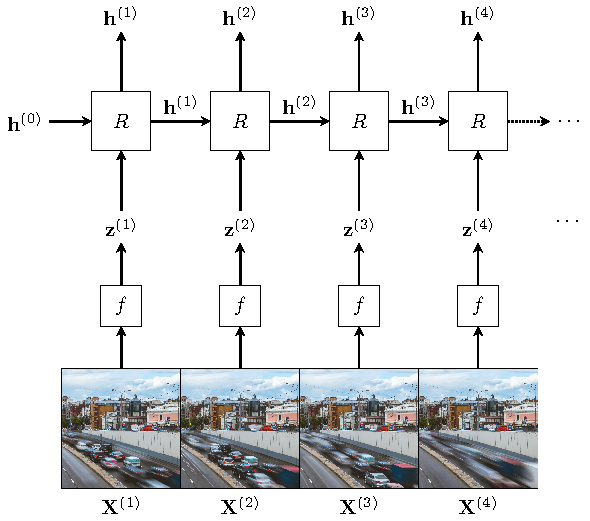
\includegraphics[width=\linewidth]{figures/normal_rnn.pdf}
    \caption{Illustration of processing video input with RNNs. Each input video frame $\vec{X}^{(t)}$ is processed using a shared function $f$---e.g. a translation invariant CNN---into a flat representation $\vec{z}^{(t)}$. Then the RNN update function $R$ is iterated across these vectors, iteratively updating a summary vector $\vec{h}^{(t)}$ which summarises all the inputs up to and including $\vec{z}^{(t)}$. The computation is seeded with an initial summary vector $\vec{h}^{(0)}$, which may be either pre-determined or learnable.}
    \label{fig:normal_rnn}
\end{figure}
At each step, the recurrent neural network computes an $m$-dimensional \emph{summary} vector $\vec{h}^{(t)}$ of all the input steps up to and
including $t$. This (partial) summary is computed conditional on the current step's
features and the previous step's summary, through a shared \emph{update} function, $R : \mathbb{R}^k \times \mathbb{R}^m \rightarrow \mathbb{R}^m$, as follows (see Figure \ref{fig:normal_rnn} for a summary):
\begin{equation}\label{eqn:rnn_upd}
    \vec{h}^{(t)} = R(\vec{z}^{(t)}, \vec{h}^{(t-1)})
\end{equation}
and, as both $\vec{z}^{(t)}$ and $\vec{h}^{(t-1)}$ are \emph{flat} vector representations, $R$ may be most easily expressed as a single fully-connected neural network layer (often known as \emph{SimpleRNN}\marginnote{In spite of their name, SimpleRNNs are remarkably expressive. For example, it was shown by \citet{siegelmann1995computational} that such models are \emph{Turing-complete}, meaning that they can likely represent \emph{any} computation we may ever be able to execute on computers.}; see \citet{elman1990finding,jordan1997serial}):
\begin{equation}\label{eqn:SimpleRNN}
     \vec{h}^{(t)} = \sigma(\vec{W}\vec{z}^{(t)} + \vec{U}\vec{h}^{(t-1)} + \vec{b})
\end{equation}
where $\vec{W}\in\mathbb{R}^{k\times m}$, $\vec{U}\in\mathbb{R}^{m\times m}$ and $\vec{b}\in\mathbb{R}^m$ are learnable parameters, and $\sigma$ is an activation function. While this introduces \emph{loops} in the network's computational graph, in practice
the network is unrolled for an appropriate number of steps, allowing for \emph{backpropagation through time} \citep{robinson1987utility,werbos1988generalization,mozer1989focused} to be applied.

The summary vectors may then be appropriately leveraged for the downstream task---if
a prediction is required at every step of the sequence, then a shared predictor may be applied
to each $\vec{h}^{(t)}$ individually. For classifying entire sequences, typically the final summary, $\vec{h}^{(T)}$, is passed to a classifier. Here, $T$ is the length of the sequence.

Specially, the initial summary vector is usually either set to the zero-vector, i.e. $\vec{h}^{(0)}=\vec{0}$, or it is made learnable. Analysing the manner in which the initial summary vector is set also allows us to deduce an interesting form of \emph{translation equivariance} exhibited by RNNs.

\paragraph{Translation equivariance in RNNs} Since we interpret the individual steps $t$ as \emph{discrete time-steps}, the input vectors $\vec{z}^{(t)}$ can be seen as living on a one-dimensional\marginnote{Note that this construction is extendable to grids in higher dimensions, allowing us to, e.g., process signals living on images in a \emph{scanline} fashion. Such a construction powered a popular series of models, such as the PixelRNN from \citet{van2016pixel}.} \emph{grid} of time-steps. While it might be attractive to attempt extending our translation equivariance analysis from CNNs here, it cannot be done in a trivial manner. 

To see why, let us assume that we have produced a new sequence $\vec{z}'^{(t)} = \vec{z}^{(t+1)}$ by performing a left-shift of our sequence by one step. %, recovering a new sequence $\vec{z}'^{(t)} = \vec{z}^{(t+1)}$. 
It might be tempting to attempt showing $\vec{h}'^{(t)} = \vec{h}^{(t+1)}$, as one expects with translation equivariance; however, this will not generally hold. Consider $t = 1$; directly applying and expanding the update function, we recover the following:
\begin{align}\label{eqn:shiftrnn}
    \vec{h}'^{(1)} &= R(\vec{z}'^{(1)}, \vec{h}^{(0)}) = R(\vec{z}^{(2)}, \vec{h}^{(0)})\\ 
    \vec{h}^{(2)} &= R(\vec{z}^{(2)}, \vec{h}^{(1)}) = R(\vec{z}^{(2)}, R(\vec{z}^{(1)}, \vec{h}^{(0)}))\label{eqn:shiftrnn2} 
\end{align}
Hence, unless we can guarantee that $\vec{h}^{(0)} = R(\vec{z}^{(1)}, \vec{h}^{(0)})$, we will not recover translation equivariance. Similar analysis can then be done for steps $t > 1$. 

Fortunately, with a slight refactoring of how we represent $\vec{z}$, and for a suitable choice of $R$, it is possible to satisfy the equality above, and hence demonstrate a setting in which RNNs are equivariant to shifts.
%
Our problem was largely one of \emph{boundary conditions}: the equality above includes $\vec{z}^{(1)}$, which our left-shift operation destroyed. To abstract this problem away, we will observe how an RNN processes an appropriately \emph{left-padded} sequence, $\bar{\vec{z}}^{(t)}$, defined as follows: 
$$
    \bar{\vec{z}}^{(t)} = \begin{cases}
        \vec{0} & t \leq t'\\
        \vec{z}^{(t - t')} & t > t' 
    \end{cases}
$$
Such a sequence now allows for left-shifting\marginnote{Note that equivalent analyses will arise if we use a different padding vector than $\vec{0}$.} by up to $t'$ steps without destroying any of the original input elements. Further, note we do not need to handle right-shifting separately; indeed, equivariance to right shifts naturally follows from the RNN equations.

We can now again analyse the operation of the RNN over a left-shifted verson of $\bar{\vec{z}}^{(t)}$, which we denote by $\bar{\vec{z}}'^{(t)} = \bar{\vec{z}}^{(t+1)}$, as we did in Equations \ref{eqn:shiftrnn}--\ref{eqn:shiftrnn2}:
\begin{align*}
    \vec{h}'^{(1)} &= R(\bar{\vec{z}}'^{(1)}, \vec{h}^{(0)}) = R(\bar{\vec{z}}^{(2)}, \vec{h}^{(0)})\\ \vec{h}^{(2)} &= R(\bar{\vec{z}}^{(2)}, \vec{h}^{(1)}) = R(\bar{\vec{z}}^{(2)}, R(\bar{\vec{z}}^{(1)}, \vec{h}^{(0)})) = R(\bar{\vec{z}}^{(2)}, R(\vec{0}, \vec{h}^{(0)}))
\end{align*}
where the substitution $\bar{\vec{z}}^{(1)} = \vec{0}$ holds as long as $t' \geq 1$, i.e. as long as any padding is applied\marginnote{In a very similar vein, we can derive equivariance to left-shifting by $s$ steps as long as $t' \geq s$.}. Now, we can guarantee equivariance to left-shifting by one step ($\vec{h}'^{(t)} = \vec{h}^{(t+1)}$) as long as $\vec{h}^{(0)} = R(\vec{0}, \vec{h}^{(0)})$.


Said differently, $\vec{h}^{(0)}$ must be chosen to be a \emph{fixed point} of a function $\gamma(\vec{h}) = R(\vec{0}, \vec{h})$. If the update function $R$ is conveniently chosen, then not only can we guarantee existence of such fixed points, but we can even directly obtain them by iterating the application of $R$ until convergence; e.g., as follows:
\begin{equation}\label{eqn:iterated}
    \vec{h}_0 = \vec{0} \qquad \vec{h}_{k+1} = \gamma(\vec{h}_{k}),
\end{equation}
%
where the index $k$ refers to the iteration of $R$ in our computation, as opposed to the the index $(t)$ denoting the time step of the RNN.  
%
If we choose $R$ such that $\gamma$ is a \emph{contraction mapping}\marginnote{Contractions are functions $\gamma: \mathcal{X}\rightarrow \mathcal{X}$ such that, under some norm $\|\cdot\|$ on $\mathcal{X}$, applying $\gamma$ \emph{contracts} the distances between points: for all $\vec{x},\vec{y}\in\mathcal{X}$, and some $q\in [0,1)$, it holds that $\|\gamma(\vec{x}) - \gamma(\vec{y})\| \leq q\|\vec{x} - \vec{y}\|$. Iterating such a function then necessarily converges to a unique fixed point, as a direct consequence of \emph{Banach's Fixed Point Theorem} \citep{banach1922operations}.}, such an iteration will indeed converge to a \emph{unique} fixed point. Accordingly, we can then iterate Equation~(\ref{eqn:iterated}) until $\vec{h}_{k+1} = \vec{h}_k$, and we can set $\vec{h}^{(0)} = \vec{h}_k$. Note that this computation is equivalent to \emph{left-padding} the sequence with ``sufficiently many'' zero-vectors.

\paragraph{Depth in RNNs} 
It is also easy to stack multiple RNNs---simply use the $\vec{h}^{(t)}$ vectors as an input sequence for a second RNN. This kind of construction is occasionally called a ``deep RNN'', which is potentially misleading. Effectively, due to the repeated application of the recurrent operation, even a single RNN ``layer'' has depth \emph{equal to the number of input steps}.

This often introduces uniquely challenging learning dynamics when optimising RNNs, as each training example induces many gradient updates to the \emph{shared} parameters of the update network. Here we will focus on perhaps the most prominent such issue---that of \emph{vanishing} and \emph{exploding} gradients \citep{bengio1994learning}---which is especially problematic in RNNs, given their depth and parameter sharing. Further, it has single-handedly spurred some of the most influential research on RNNs. For a more detailed overview, we refer the reader to \citet{pascanu2013difficulty}, who have studied the training dynamics of RNNs in great detail, and exposed these challenges from a variety of perspectives: analytical, geometrical, and the lens of dynamical systems.

To illustrate vanishing gradients, consider a SimpleRNN with a sigmoidal activation function  $\sigma$\marginnote{\includegraphics[width=\linewidth]{figures/sigmoid.pdf}\\ Examples of such an activation include the \emph{logistic function}, $\sigma(x) = \frac{1}{1+\exp(-x)}$, and the \emph{hyperbolic tangent}, $\sigma(x)=\tanh x$. They are called sigmoidal due to the distinct S-shape of their plots.}, whose derivative magnitude $|\sigma'|$ is always between $0$ and $1$. Multiplying many such values results in gradients that quickly tend to zero, implying that early steps in the input sequence may not be able to have influence in updating the network parameters at all.

For example, consider the next‐word prediction task (common in e.g. predictive keyboards), and the input text \emph{``Petar is Serbian. He was born on \dots [long paragraph] \dots Petar currently lives in \rule{1.3cm}{0.15mm}''}. Here, predicting the next word as ``Serbia'' may only be reasonably concluded by considering the very start of the paragraph—but gradients have likely vanished by the time they reach this input step, making learning from such examples very challenging.

Deep feedforward neural networks have also suffered from the vanishing gradient problem, until the invention of the ReLU activation (which has gradients equal to \emph{exactly} zero or one---thus fixing the vanishing gradient problem). However, in RNNs, using ReLUs may easily lead to \emph{exploding} gradients, as the output space of the update function is now \emph{unbounded}, and gradient descent will update the cell once for every input step, quickly building up the scale of the updates.
%
Historically, the vanishing gradient phenomenon was recognised early on as a significant obstacle in the use of recurrent networks. Coping with this problem motivated the development of more sophisticated RNN layers, which we describe next.


\subsection{Long Short-Term Memory networks}
\label{sec:lstm}

\begin{figure}
    \centering
    \includegraphics[width=\linewidth]{figures/lstm.pdf}
    \caption{The dataflow of the long short-term memory (LSTM), with its components and memory cell ($M$) clearly highlighted. Based on the current input $\vec{z}^{(t)}$, previous summary $\vec{h}^{(t-1)}$ and previous cell state $\vec{c}^{(t-1)}$, the LSTM predicts the updated cell state $\vec{c}^{(t)}$ and summary $\vec{h}^{(t)}$.}
    \label{fig:lstm}
\end{figure}
A key invention that significantly reduced the effects of vanishing gradients in RNNs is that of \emph{gating mechanisms}, which allow the network to selectively \emph{overwrite} information in a data-driven way. Prominent examples of these \emph{gated RNNs} include the {\em Long Short-Term Memory} (LSTM; \citet{hochreiter1997long}) and the {\em Gated Recurrent Unit} (GRU; \citet{cho2014learning}). Here we will primarily discuss the LSTM---specifically, the variant presented by \citet{graves2013generating}---in order to illustrate the operations of such models. Concepts from LSTMs easily carry over to other gated RNNs.

Throughout this section, it will likely be useful to refer to Figure \ref{fig:lstm}, which illustrates all of the LSTM operations that we will discuss in text.

The LSTM augments the recurrent computation by introducing a \emph{memory cell}, which stores \emph{cell state} vectors, $\vec{c}^{(t)}\in\mathbb{R}^m$, that are \emph{preserved} between computational steps. The LSTM computes summary vectors, $\vec{h}^{(t)}$, directly based on $\vec{c}^{(t)}$, and $\vec{c}^{(t)}$ is, in turn, computed using $\vec{z}^{(t)}$, $\vec{h}^{(t-1)}$ and $\vec{c}^{(t-1)}$.
Critically, the cell is \textbf{not} completely overwritten based on $\vec{z}^{(t)}$ and $\vec{h}^{(t-1)}$, which would expose the network to the same issues as the SimpleRNN. Instead, a certain quantity of the previous cell state may be \emph{retained}---and the proportion by which this occurs is explicitly \emph{learned} from data.

Just like in SimpleRNN, we compute features by using a single fully-connected neural network layer over the current input step and previous summary:\marginnote{Note that we have set the activation function to $\tanh$ here; as LSTMs are designed to ameliorate the vanishing gradient problem, it is now appropriate to use a sigmoidal activation.}
\begin{equation}\label{eqn:lstmstart}
     \widetilde{\vec{c}}^{(t)} = \tanh(\vec{W}_c\vec{z}^{(t)} + \vec{U}_c\vec{h}^{(t-1)} + \vec{b}_c)
\end{equation}
But, as mentioned, we do not allow \emph{all} of this vector to enter the cell---hence why we call it the vector of \emph{candidate} features, and denote it as $\widetilde{\vec{c}}^{(t)}$. Instead, the LSTM directly learns \emph{gating vectors}, which are real-valued vectors in the range $[0, 1]$, and decide how much of the signal should be allowed to enter, exit, and overwrite the memory cell. 

Three such gates are computed, all based on $\vec{z}^{(t)}$ and $\vec{h}^{(t-1)}$: the \emph{input gate} $\vec{i}^{(t)}$, which computes the proportion of the candidate vector allowed to enter the cell; the \emph{forget gate} $\vec{f}^{(t)}$, which computes the proportion of the previous cell state to be retained, and the \emph{output gate} $\vec{o}^{(t)}$, which computes the proportion of the new cell state to be used for the final summary vector. Typically all of these gates are also derived using a single fully connected layer, albeit with the \emph{logistic sigmoid} activation $\mathrm{logistic}(x) = \frac{1}{1+\exp(-x)}$, in order to guarantee that the outputs are in the $[0, 1]$ range\marginnote{Note that the three gates are themselves \emph{vectors}, i.e. $\vec{i}^{(t)}, \vec{f}^{(t)}, \vec{o}^{(t)}\in [0,1]^m$. This allows them to control how much \emph{each} of the $m$ dimensions is allowed through the gate.}:
\begin{align}\label{eqn:lstm_gate}
     \vec{i}^{(t)} &= \mathrm{logistic}(\vec{W}_\mathrm{i}\vec{z}^{(t)} + \vec{U}_\mathrm{i}\vec{h}^{(t-1)} + \vec{b}_\mathrm{i})\\
     \vec{f}^{(t)} &= \mathrm{logistic}(\vec{W}_\mathrm{f}\vec{z}^{(t)} + \vec{U}_\mathrm{f}\vec{h}^{(t-1)} + \vec{b}_\mathrm{f})\\
     \vec{o}^{(t)} &= \mathrm{logistic}(\vec{W}_\mathrm{o}\vec{z}^{(t)} + \vec{U}_\mathrm{o}\vec{h}^{(t-1)} + \vec{b}_\mathrm{o})
\end{align}

Finally, these gates are appropriately applied to decode the \emph{new} cell state, $\vec{c}^{(t)}$, which is then modulated by the output gate to produce the summary vector $\vec{h}^{(t)}$, as follows:
\begin{align}
    \vec{c}^{(t)} &= \vec{i}^{(t)}\odot\widetilde{\vec{c}}^{(t)} + \vec{f}^{(t)}\odot\vec{c}^{(t-1)}\\
    \vec{h}^{(t)} &= \vec{o}^{(t)}\odot\tanh(\vec{c}^{(t)})\label{eqn:lstm_end}
\end{align}
where $\odot$ is element-wise vector multiplication. Applied together, Equations (\ref{eqn:lstmstart})--(\ref{eqn:lstm_end}) completely specify the \emph{update rule} for the LSTM, which now takes into account the cell vector $\vec{c}^{(t)}$ as well\marginnote{This is still compatible with the RNN update blueprint from Equation (\ref{eqn:rnn_upd}); simply consider the summary vector to be the \emph{concatenation} of $\vec{h}^{(t)}$ and $\vec{c}^{(t)}$; sometimes denoted by $\vec{h}^{(t)}\|\vec{c}^{(t)}$.}:
$$
    (\vec{h}^{(t)}, \vec{c}^{(t)}) = R(\vec{z}^{(t)}, (\vec{h}^{(t-1)}, \vec{c}^{(t-1)}))
$$
Note that, as the values of $\vec{f}^{(t)}$ are derived from $\vec{z}^{(t)}$ and $\vec{h}^{(t-1)}$---and therefore directly \emph{learnable} from data---the LSTM effectively learns how to appropriately forget past experiences. Indeed, the values of $\vec{f}^{(t)}$ directly appear in the backpropagation update for all the LSTM parameters ($\vec{W}_*, \vec{U}_*, \vec{b}_*$), allowing the network to explicitly \emph{control}, in a data-driven way, the degree of vanishing for the gradients across the time steps.

Besides tackling the vanishing gradient issue head-on, it turns out that gated RNNs also unlock a very useful form of invariance to \emph{time-warping} transformations, which remains out of reach of SimpleRNNs.

\paragraph{Time warping invariance of gated RNNs} We will start by illustrating, in a \emph{continuous-time} setting\marginnote{We focus on the continuous setting as it will be easier to reason about manipulations of time there.}, what does it mean to \emph{warp time}, and what is required of a recurrent model in order to achieve invariance to such transformations. Our exposition will largely follow the work of \citet{tallec2018can}, that initially described this phenomenon---and indeed, they were among the first to actually study RNNs from the lens of invariances.

Let us assume a continuous time-domain signal $z(t)$, on which we would like to apply an RNN. To align the RNN's discrete-time computation of summary vectors $\vec{h}^{(t)}$\marginnote{We will use $h(t)$ to denote a continuous signal at time $t$, and $\vec{h}^{(t)}$ to denote a discrete signal at time-step $t$.} with an analogue in the continuous domain, $h(t)$, we will observe its linear Taylor expansion:
\begin{equation}
    h(t + \delta) \approx h(t) + \delta\frac{\mathrm{d}h(t)}{\mathrm{d}t}
\end{equation}
and, setting $\delta = 1$, we recover a relationship between $h(t)$ and $h(t+1)$, which is exactly what the RNN update function $R$ (Equation \ref{eqn:rnn_upd}) computes. Namely, the RNN update function satisfies the following differential equation:
\begin{equation}\label{eqn:ode_pre_warp}
    \frac{\mathrm{d}h(t)}{\mathrm{d}t} = h(t+1) - h(t) = R(z(t+1), h(t)) - h(t)
\end{equation}

We would like the RNN to be resilient to the way in which the signal is sampled (e.g. by changing the time unit of measurement), in order to account for any imperfections or irregularities therein. Formally, we denote a \emph{time warping}\marginnote{\includegraphics[width=\linewidth]{figures/time_warp.pdf}\\ Such warping operations can be \emph{simple}, such as time rescaling; e.g. $\tau(t) = 0.7t$ (displayed above), which, in a discrete setting, would amount to new inputs being received every $\sim 1.43$ steps. However, it also admits a wide spectrum of \emph{variably-changing} sampling rates, e.g. sampling may freely accelerate or decelerate throughout the time domain.} operation $\tau : \mathbb{R}^+\rightarrow\mathbb{R}^+$, as any monotonically increasing differentiable mapping between times. The notation $\tau$ is chosen because time warping represents an \emph{automorphism} of time.

Further, we state that a class of models is \emph{invariant} to time warping if, for any model of the class and any such $\tau$, there exists another (possibly the same) model from the class that processes the warped data in the same way as the original model did in the non-warped case.

This is a potentially very useful property. If we have an RNN class capable of modelling short-term dependencies well, and we can also show that this class is invariant to time warping, then we know it is possible to train such a model in a way that will usefully capture long-term dependencies as well (as they would correspond to a time dilation warping of a signal with short-term dependencies). 
%
As we will shortly see, it is no coincidence that \emph{gated} RNN models such as the LSTM were proposed to model long-range dependencies. Achieving time warping invariance is tightly coupled with presence of gating mechanisms, such as the input/forget/output gates of LSTMs.

When time gets warped by $\tau$, the signal observed by the RNN at time $t$ is $z(\tau(t))$ and, to remain invariant to such warpings, it should predict an equivalently-warped summary function $h(\tau(t))$. Using Taylor expansion arguments once more, we derive a form of Equation \ref{eqn:ode_pre_warp} for the warped time, that the RNN update $R$ should satisfy:
\begin{equation}\label{eqn:ode_post_warp}
    \frac{\mathrm{d}h(\tau(t))}{\mathrm{d}\tau(t)} = R(z(\tau(t+1)), h(\tau(t))) - h(\tau(t))
\end{equation}
However, the above derivative is computed with respect to the warped time $\tau(t)$, and hence does not take into account the original signal. To make our model take into account the warping transformation explicitly, we need to differentiate the warped summary function with respect to $t$. Applying the chain rule, this yields the following differential equation:
\begin{equation}\label{eqn:full_ode_warp}
    \frac{\mathrm{d}h(\tau(t))}{\mathrm{d}t} = \frac{\mathrm{d}h(\tau(t))}{\mathrm{d}\tau(t)}\frac{\mathrm{d}\tau(t)}{\mathrm{d}t} = \frac{\mathrm{d}\tau(t)}{\mathrm{d}t}R(z(\tau(t+1)), h(\tau(t))) - \frac{\mathrm{d}\tau(t)}{\mathrm{d}t}h(\tau(t))
\end{equation}
and, for our (continuous-time) RNN to remain invariant to \emph{any} time warping $\tau(t)$, it needs to be able to explicitly represent the derivative $\frac{\mathrm{d}\tau(t)}{\mathrm{d}t}$, which is not assumed known upfront! We need to introduce a \emph{learnable} function $\Gamma$ which approximates this derivative. For example, $\Gamma$ could be a neural network taking into account $z(t+1)$ and $h(t)$ and predicting scalar outputs.

Now, remark that, from the point of view of a \emph{discrete} RNN model under time warping, its input $\vec{z}^{(t)}$ will correspond to $z(\tau(t))$, and its summary $\vec{h}^{(t)}$ will correspond to $h(\tau(t))$. To obtain the required relationship of $\vec{h}^{(t)}$ to $\vec{h}^{(t+1)}$ in order to remain invariant to time warping, we will use a one-step Taylor expansion of $h(\tau(t))$:
\begin{equation*}
    h(\tau(t + \delta)) \approx h(\tau(t)) + \delta\frac{\mathrm{d}h(\tau(t))}{\mathrm{d}t}
\end{equation*}
and, once again, setting $\delta=1$ and substituting Equation \ref{eqn:full_ode_warp}, then discretising:
\begin{align*}
    \vec{h}^{(t+1)} &= \vec{h}^{(t)} + \frac{\mathrm{d}\tau(t)}{\mathrm{d}t}R(\vec{z}^{(t+1)}, \vec{h}^{(t)}) - \frac{\mathrm{d}\tau(t)}{\mathrm{d}t}\vec{h}^{(t)}\\
    &= \frac{\mathrm{d}\tau(t)}{\mathrm{d}t}R(\vec{z}^{(t+1)}, \vec{h}^{(t)}) + \left(1 - \frac{\mathrm{d}\tau(t)}{\mathrm{d}t}\right)\vec{h}^{(t)}
\end{align*}
Finally, we swap $\frac{\mathrm{d}\tau(t)}{\mathrm{d}t}$ with the aforementioned learnable function, $\Gamma$. This gives us the required form for our time warping-invariant RNN:
\begin{equation}\label{eqn:GaRNN}
    \vec{h}^{(t+1)} = \Gamma(\vec{z}^{(t+1)}, \vec{h}^{(t)})R(\vec{z}^{(t+1)}, \vec{h}^{(t)}) + (1 - \Gamma(\vec{z}^{(t+1)}, \vec{h}^{(t)}))\vec{h}^{(t)}
\end{equation}
We may quickly deduce that SimpleRNNs (Equation \ref{eqn:SimpleRNN}) are \emph{not} time warping invariant, given that they do not feature the second term in Equation \ref{eqn:GaRNN}. Instead, they fully overwrite $\vec{h}^{(t)}$ with $R(\vec{z}^{(t+1)}, \vec{h}^{(t)})$, which corresponds to assuming no time warping at all; $\frac{\mathrm{d}\tau(t)}{\mathrm{d}t} = 1$, i.e. $\tau(t) = t$.

Further, our link between continuous-time RNNs and the discrete RNN based on $R$ rested on the accuracy of the Taylor approximation, which holds only if the time-warping derivative is not too large, i.e., $\frac{\mathrm{d}\tau(t)}{\mathrm{d}t}\lesssim 1$. The intuitive explanation of this is: if our time warping operation ever \emph{contracts time} in a way that makes time increments ($t \rightarrow t + 1$) large enough that intermediate data changes are not sampled, the model can never hope to process time-warped inputs in the same way as original ones---it simply would not have access to the same information. Conversely, time \emph{dilations} of any form (which, in discrete terms, correspond to interspersing the input time-series with zeroes) are perfectly allowed within our framework.

Combined with our requirement of monotonically increasing $\tau$ ($\frac{\mathrm{d}\tau(t)}{\mathrm{d}t} > 0$), we can bound the output space of $\Gamma$ as $0 < \Gamma(\vec{z}^{(t+1)}, \vec{h}^{(t)}) < 1$, which motivates the use of the logistic sigmoid activation for $\Gamma$, e.g.:
$$
    \Gamma(\vec{z}^{(t+1)}, \vec{h}^{(t)}) = \mathrm{logistic}({\bf W}_\Gamma\vec{z}^{(t+1)} + {\bf U}_\Gamma\vec{h}^{(t)} + \vec{b}_\Gamma)
$$
\emph{exactly} matching the LSTM gating equations (e.g. Equation \ref{eqn:lstm_gate}). The main difference is that LSTMs compute gating \emph{vectors}, whereas Equation \ref{eqn:GaRNN} implies $\Gamma$ should output a scalar. Vectorised gates \citep{hochreiter1991untersuchungen} allow to fit a \emph{different} warping derivative in every dimension of $\vec{h}^{(t)}$, allowing for reasoning over \emph{multiple} time horizons simultaneously.

It is worth taking a pause here to summarise what we have done. By requiring that our RNN class is invariant to (non-destructive) time warping, we have derived the necessary form that it must have (Equation \ref{eqn:GaRNN}), and showed that it exactly corresponds to the class of \emph{gated} RNNs. The gates' primary role under this perspective is to accurately fit the \emph{derivative} $\frac{\mathrm{d}\tau(t)}{\mathrm{d}t}$ of the warping transformation.

The notion of \emph{class invariance} is somewhat distinct from the invariances we studied previously. Namely, once we train a gated RNN on a time-warped input with $\tau_1(t)$, we typically cannot zero-shot transfer\marginnote{One case where zero-shot transfer is possible is when the second time warping is assumed to be a \emph{time rescaling} of the first one ($\tau_2(t) = \alpha\tau_1(t)$). Transferring a gated RNN pre-trained on $\tau_1$ to a signal warped by $\tau_2$ merely requires \emph{rescaling the gates}: $\Gamma_2(\vec{z}^{(t+1)}, \vec{h}^{(t)}) = \alpha \Gamma_1(\vec{z}^{(t+1)}, \vec{h}^{(t)})$. $R$ can retain its parameters ($R_1 = R_2$).} it to a  signal warped by a different $\tau_2(t)$. Rather, class invariance only guarantees that gated RNNs are powerful enough to fit both of these signals in the same manner, but potentially with vastly different model parameters. That being said, the realisation that effective gating mechanisms are tightly related to fitting the warping derivative can yield useful prescriptions for gated RNN optimisation, as we now briefly demonstrate.

For example, we can often assume that the range of the dependencies we are interested in tracking within our signal will be in the range $[T_l, T_h]$ time-steps.

By analysing the analytic solutions to Equation \ref{eqn:full_ode_warp}, it can be shown that the characteristic \emph{forgetting time} of $\vec{h}^{(t)}$ by our gated RNN is proportional to $\frac{1}{\Gamma(\vec{z}^{(t+1)}, \vec{h}^{(t)})}$. Hence, we would like our gating values to lie between $\left[\frac{1}{T_h}, \frac{1}{T_m}\right]$ in order to effectively remember information within the assumed range.

Further, if we assume that $\vec{z}^{(t)}$ and $\vec{h}^{(t)}$ are roughly \emph{zero-centered}---which is a common by-product of applying transformations such as layer normalisation \citep{ba2016layer}---we can assume that $\mathbb{E}[\Gamma(\vec{z}^{(t+1)}, \vec{h}^{(t)})] \approx \mathrm{logistic}(\vec{b}_\Gamma)$. Controlling the \emph{bias} vector of the gating mechanism is hence a very powerful way of controlling the effective gate value\marginnote{This insight was already spotted by \citet{gers2000recurrent,jozefowicz2015empirical}, who empirically recommended initialising the forget-gate bias of LSTMs to a constant positive vector, such as $\vec{1}$.}.

Combining the two observations, we conclude that an appropriate range of gating values can be obtained by initialising $\vec{b}_\Gamma\sim-\log(\mathcal{U}(T_l, T_h) - 1)$, where $\mathcal{U}$ is the uniform real distribution. Such a recommendation was dubbed \emph{chrono initialisation} by \citet{tallec2018can}, and has been empirically shown to improve the long-range dependency modelling of gated RNNs.

\paragraph{Sequence-to-sequence learning with RNNs}
One prominent historical example of using RNN-backed computation are \emph{sequence-to-sequence} translation tasks, such as {\em machine translation} of natural languages. The pioneering \emph{seq2seq} work by \citet{sutskever2014sequence} achieved this by passing the summary vector, $\vec{h}^{(T)}$ as an initial input for a \emph{decoder} RNN, with outputs of RNN blocks being given as inputs for the next step.

\begin{figure}
    \centering
    \includegraphics[width=\linewidth]{figures/bottle_rnn.pdf}
    \caption{One typical example of a seq2seq architecture with an RNN encoder $R_\mathrm{enc}$ and RNN decoder $R_\mathrm{dec}$. The decoder is seeded with the final summary vector $\vec{h}^{(T)}$ coming out of the encoder, and then proceeds in an \emph{autoregressive} fashion: at each step, the predicted output from the previous step is fed back as input to $R_\mathrm{dec}$. The bottleneck problem is also illustrated with the red lines: the summary vector $\vec{h}^{(T)}$ is pressured to store \emph{all} relevant information for translating the input sequence, which becomes increasingly challenging as the input length grows.}
    \label{fig:rnn_bottleneck}
\end{figure}

This placed substantial representational pressure on the summary vector, $\vec{h}^{(T)}$. Within the context of deep learning, $\vec{h}^{(T)}$ is sometimes referred to as a \emph{bottleneck}\marginnote{\includegraphics[width=\linewidth]{figures/bottleneck.png}\\
The bottleneck effect has recently received substantial attention in the graph representation learning community \citep{alon2020bottleneck}, as well as neural algorithmic reasoning \citep{cappart2021combinatorial}.}. Its fixed capacity must be sufficient for representing the content of the entire input sequence, in a manner that is conducive to generating a corresponding sequence, while also supporting input sequences of substantially different lengths (Figure \ref{fig:rnn_bottleneck}).

In reality, different steps of the output may wish to focus (\emph{attend}) on different parts of the input, and all such choices are difficult to represent via a bottleneck vector. Following from this observation, the popular \emph{recurrent attention} model was proposed by \citet{bahdanau2014neural}. At every step of processing, a \emph{query vector} is generated by an RNN; this query vector then interacts with the representation of \emph{every} time-step $\vec{h}^{(t)}$, primarily by computing a weighted sum over them. This model pioneered neural content-based attention and predates the success of the Transformer model.

Lastly, while attending offers a \emph{soft} way to dynamically focus on parts of the input content, substantial work also learnt more \emph{explicit} ways to direct attention to the input. A powerful algorithmically grounded way of doing so is the \emph{pointer network} of \citet{vinyals2015pointer}, which proposes a simple modification of recurrent attention to allow for pointing over elements of \emph{variable-sized} inputs. These findings have then been generalised to the \emph{set2set} architecture \citep{vinyals2016order}, which generalises seq2seq models to unordered sets, supported by pointer network-backed LSTMs.